\chapter{True triaxial experiments}\label{ch4:title}

The development of a successful failure criterion requires experiments and particularly multi-axial testing \cite{Labuz2018} to be performed. These tests are needed to provide material performance at various stress states, e.g. to assess the intermediate principal stress effect and to enrich the database used to calibrate failure criteria. This chapter presents the multi axial experiments performed for this study. 


\section{Introduction}

The development of failure criteria requires a diversity of experiments to be the representative of the rock behavior. Axisymmetric or conventional triaxial experiments, presented in Chapter \ref{ch3:title}, are typical laboratory techniques performed as a first approach to determine strength parameters. Although they are convenient to perform, the principal stresses cannot be varied independently; two principal stresses are always equal. To address this issue, true triaxial testing was developed to represent the in-situ stress state underground, by creating “true triaxial” testing conditions that simulate three-dimensional states of stress \cite{Labuz2018} .

In addition to the three-dimensional state of stress, many geo-engineering problems approximate a plane state of strain. It is particularly the case for tunnels and other long structures with a constant cross-section and loaded in the plane of the cross-section \cite{Jaeger1979}. Although plane strain is a reasonable model of reality, the condition is challenging to reproduce in experiments. Indeed, on top of independent application of the three principal stresses, the plane-strain condition requires a precise control of the strain in the intermediate stress direction, as it should be equal to zero for the duration of the test. 

In this study, the Plane-Strain Apparatus developed by Labuz et al. (1996) \cite{Labuz1996} was selected to perform experiments on Dunnville Sandstone, as it enables experiments to be performed under a three-dimensional stress state, with the option of restricting strain in one direction.

\section{Plane-Strain Apparatus}

The University of Minnesota Plane-Strain Apparatus enables independent application of the principal stresses, using a stiff biaxial frame to induce the intermediate stress through passive restraint \cite{Labuz1996}. Recent modifications of the device enable control and monitoring of the three stresses \cite{Zeng2019}.

\subsection{Development of the apparatus}

The Plane-Strain Apparatus (US Patent number 5 063 785), was first designed based on a passive, stiff frame concept. The device enabled testing of rock specimen under plane strain conditions with active application of the major and minor stresses, and passive restraint for the intermediate stress through the biaxial frame \cite{Labuz1996}. 

The apparatus was recently improved with the addition of two hydraulic pistons acting in the intermediate principal stress direction which enable the active application and control of major, intermediate and minor stresses \cite{Zeng2019}. This device allows failure surfaces to develop and propagate in an unrestricted manner, unlike conventional triaxial compression where the specimen is constrained by the loading platens. In short, the Plane-Strain Apparatus gives the possibility to simulate in-situ conditions of rock underground. 

\subsection{Description of the apparatus}

The apparatus can be defined as a pressure cell made of four components, each one related to a particular feature of the testing conditions \cite{Labuz1996,Zeng2019}. 

\paragraph{Base unit} 
The base unit is equipped with high-pressure pass throughs designed to receive in-vessel instrumentation such as LVDTs (Linear Variable Differential Transformer), strain gages, and an internal load cell, above which specimen is placed. Figure \ref{fig4:1} shows the base unit and denotes its components. 

\begin{figure}[p]
    \centering
    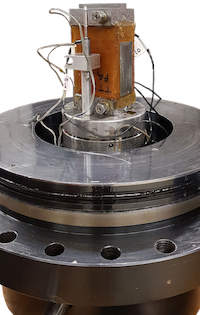
\includegraphics[width=0.4\columnwidth]{ch4/baseunite}
    \caption{Base unit of the Plane-Strain Apparatus}
    \label{fig4:1}
\end{figure} 

\paragraph{Biaxial frame}
The biaxial frame was designed to bring maximum possible stiffness to the apparatus when it was used as passive restraint to restrict deformation of the specimen. It is now hosting the hydraulic pistons, with a maximum capacity of \SI{69}{MPa}, that directly induce the intermediate stress. The frame is placed so that the pistons are aligned with the lateral platens fixed to the specimen. Two holes were machined in the frame to allow placement of the lateral LVDTs. Figure \ref{fig4:2} shows the biaxial frame and denotes its components. 


\begin{figure}[p]
    \centering
    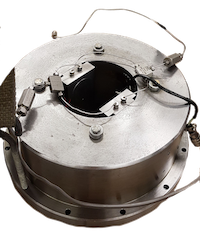
\includegraphics[width=0.4\columnwidth]{ch4/biaxialframe}
    \caption{Biaxial Frame of the Plane-Strain Apparatus}
    \label{fig4:2}
\end{figure} 

\paragraph{Loading piston assembly} 
The loading piston assembly combines two features of the apparatus. It is used to apply the axial load to the specimen and enables the failure surface to develop and propagate freely in the minor stress direction. It is composed of a linear bearing, bolted to the bottom of the loading piston, which can slide over a trackway when a mechanism forms. The loading piston maximum capacity is \SI{500}{MPa}. Figure \ref{fig4:3} shows the loading piston assembly and denotes its components.


\begin{figure}[p]
    \centering
    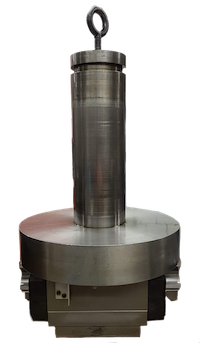
\includegraphics[width=0.4\columnwidth]{ch4/loadingpiston}
    \caption{Loading piston of the Plane-Strain Apparatus}
    \label{fig4:3}
\end{figure} 

\paragraph{Pressure vessel} The four elements presented are placed in a pressure vessel designed to hold the pressurized fluid used to apply the minor stress. The top cap and base pot are bolted to the pressure vessel surrounding the apparatus. The maximum capacity is \SI{24}{MPa}. Figure \ref{fig4:4} shows the pressure vessel and denotes its components.


\begin{figure}[p]
    \centering
    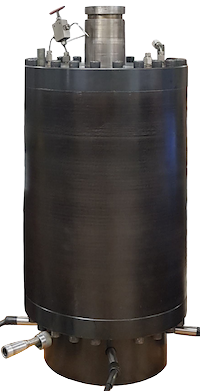
\includegraphics[width=0.3\columnwidth]{ch4/cell}
    \caption{Pressure cell of the Plane-Strain Apparatus}
    \label{fig4:4}
\end{figure} 

\section{Specimen preparation}

The concept of multi axial testing involves the use of a prismatic specimen. Indeed, in order to respect their independence, each of the three principal stresses have to be applied perpendicular to the specimen surface. The specimen preparation included geometric adjustments, instrumentation with strain gages, and jacketing. 

\subsection{Dimensions}

The theoretical dimensions of the specimen used for true-triaxial testing in the Plane-Strain Apparatus are presented in the Figure \ref{fig4:5}. 

\begin{figure}[tb]
    \centering
    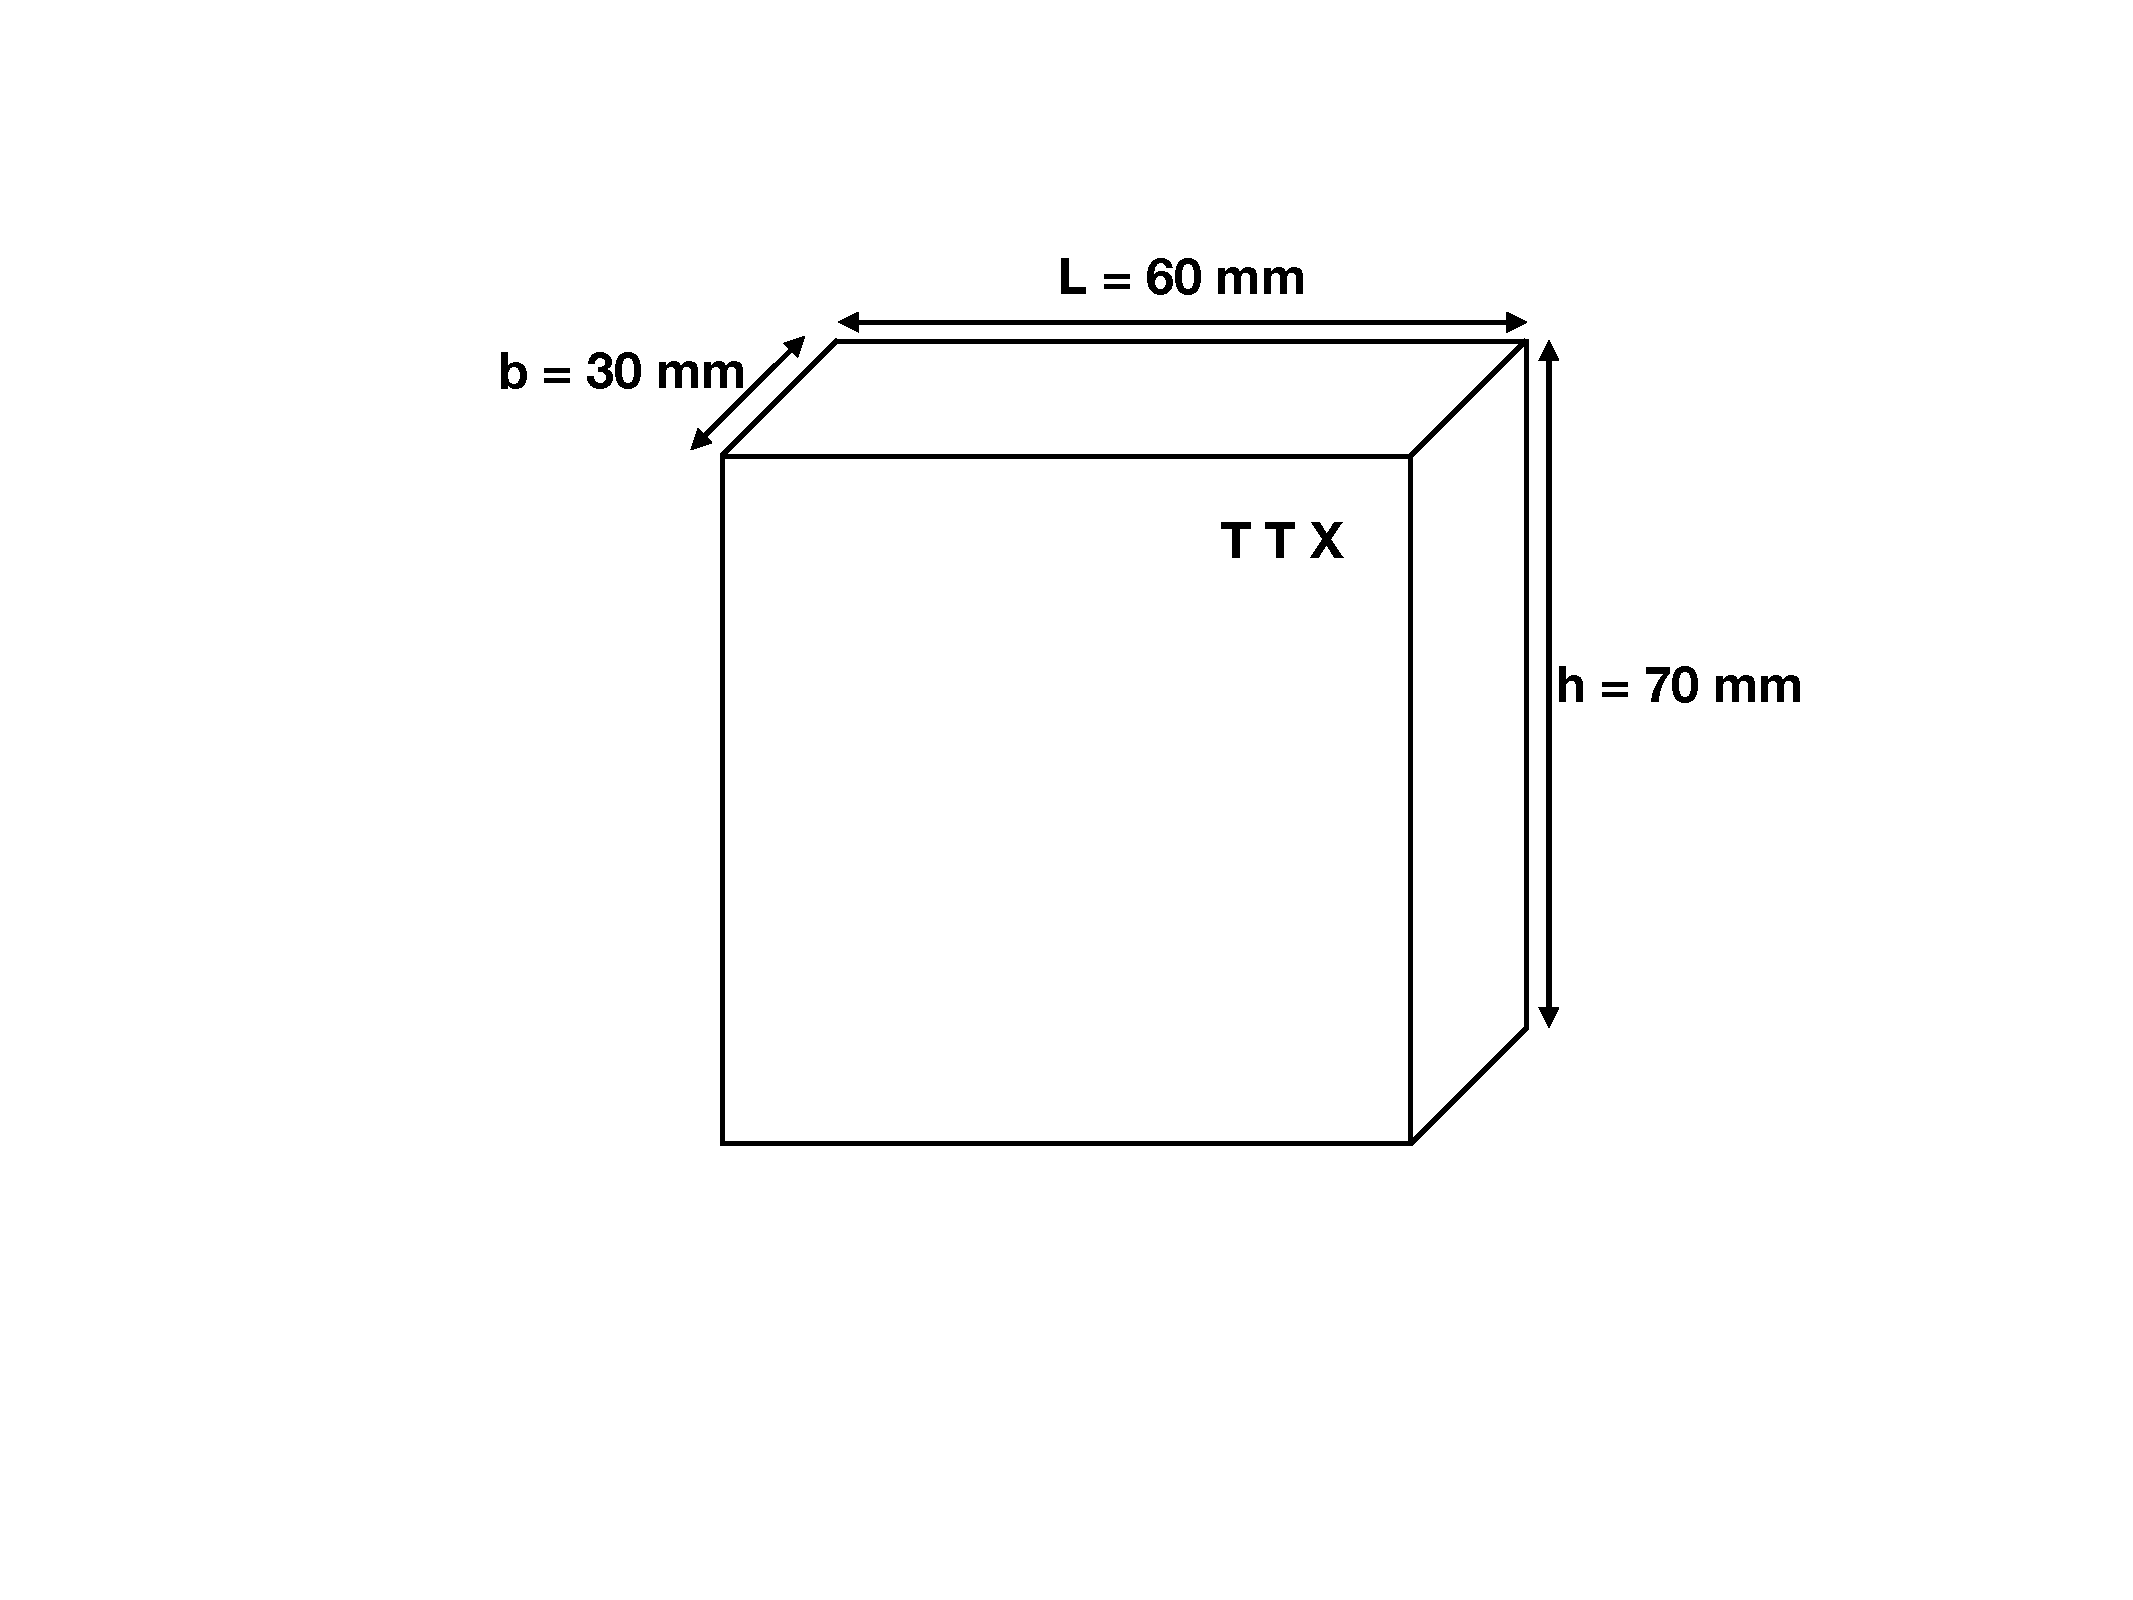
\includegraphics[width=0.4\columnwidth]{ch4/dimensions.pdf}
    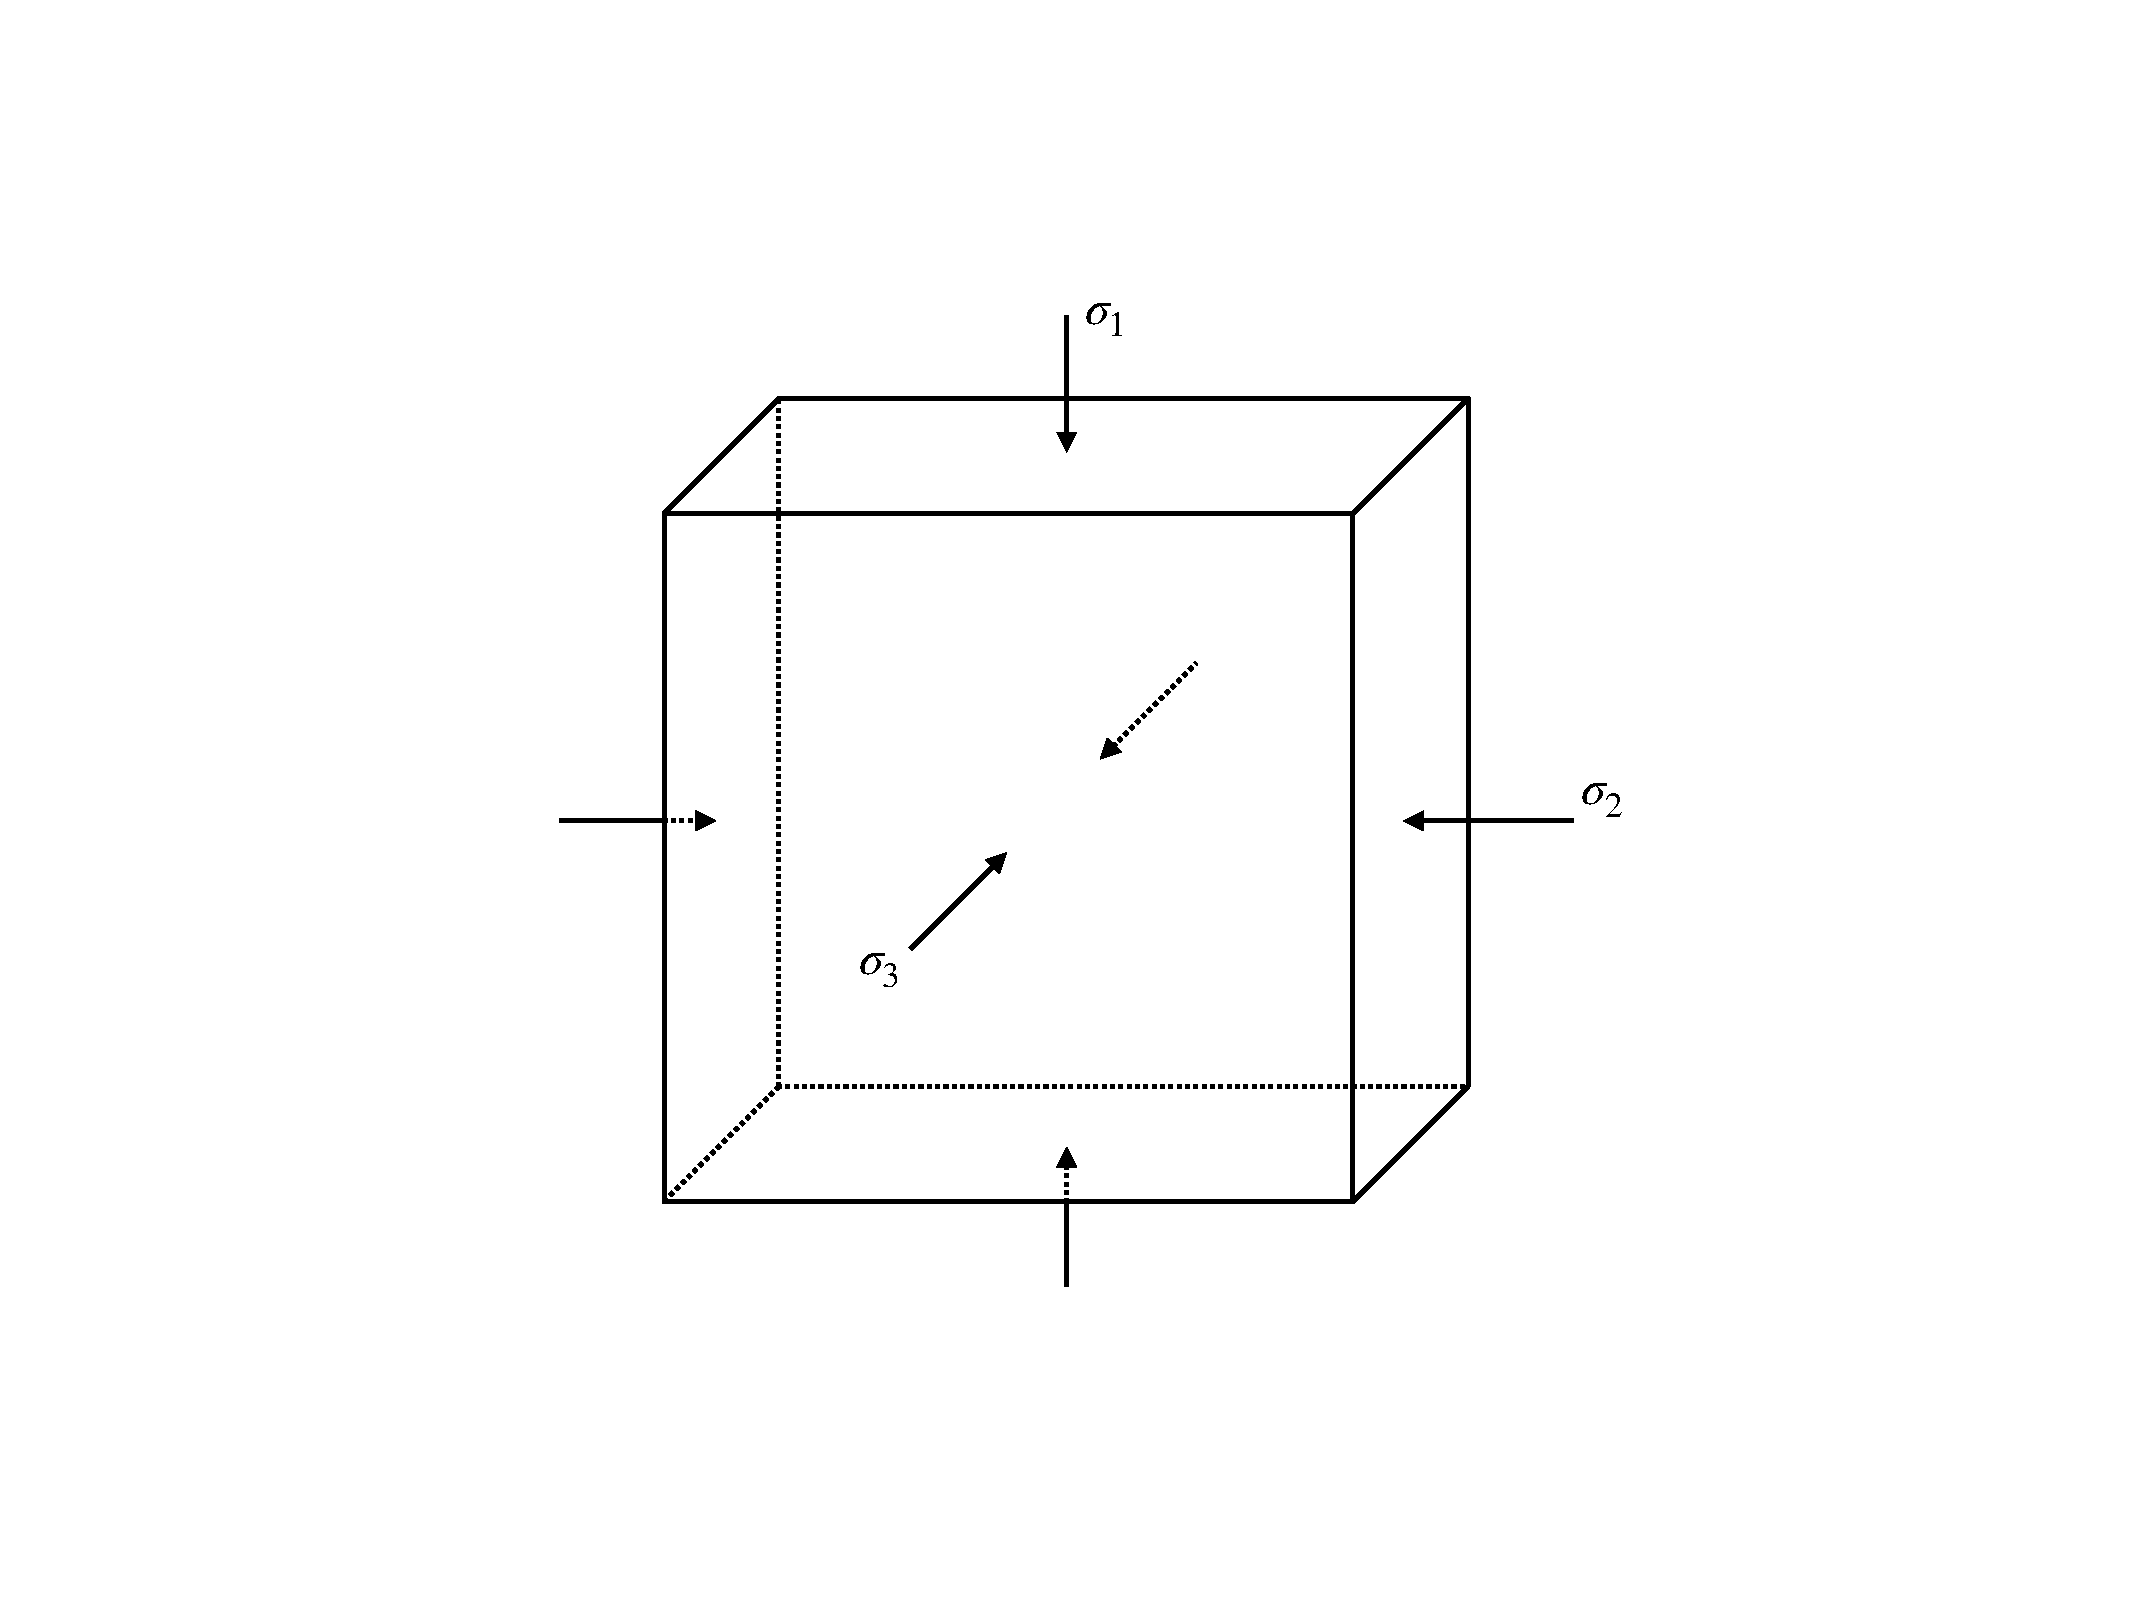
\includegraphics[width=0.4\columnwidth]{ch4/spestate}
    \caption{a. Specimen dimensions and b. loading directions}
    \label{fig4:5}
\end{figure} 

Four prismatic specimens were obtained from a block of Dunnville sandstone to minimize variation in properties. In preparation of the test specimens, particular attention was given to (i) the straightness of the elements on the cylindrical surface, (ii) flatness of the end bearing surfaces and (iii) perpendicularity of the end surfaces with the respect to axis of the core. In order to adjust the dimensions and to ensure (i), (ii) and (iii), the specimens were ground according to the ISRM suggested methods \cite{ISRM2015} and the ASTM standard \cite{ASTM2019}. A detailed description of the specimen preparation procedure is presented in section \ref{Conventional_Triaxial_tests}. The final dimensions for the four specimens tested were: $h=\SI{69+-1}{\milli\meter}$, $L=\SI{60+-1}{\milli\meter}$, 
$b=\SI{30+-0.5}{\milli\meter}$.

The true-triaxial experiments, in the Plane Strain Apparatus, are performed on dry specimens (drained conditions). After the geometry adjustment, the specimens were oven dried for 24 hours at \SI{100}{\celsius}.

\subsection{Specimen instrumentation}

Strain measurements in the three principal directions are needed to analyze the volume change behavior of the rock specimen during the experiment. These measurements were made using strain gages as part of the instrumentation setup for multi axial tests. 

One face of the specimens was equipped with a pair of strain gages made of one for axial strain and the other for transversal strain measurements. The set-up procedure is the same as the one described in section \ref{Conventional_Triaxial_tests}. Once the strain gages were fixed (24 hours of drying), the lead wires were soldered. Figure \ref{fig4:6} shows the instrumentation of specimen “TT2”.  

\begin{figure}[tb]
    \centering
    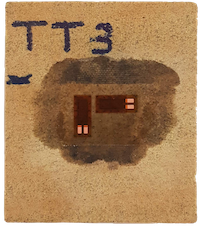
\includegraphics[width=0.4\columnwidth]{ch4/specimen}
    \caption{Specimen instrumented with axial and transversal strain gages}
    \label{fig4:6}
\end{figure} 

\subsection{Jacketing}

During an experiment in the Plane-Strain Apparatus, the specimen and the instrumentation are immersed in oil used to apply one of the lateral stresses. As the true-triaxial experiments were performed under drained conditions, the specimen needed to be dry (drained) for the duration of the test. 

The specimen is protected from the oil by a polyurethane membrane that include the top, bottom and lateral platens in contact with the specimen (Figure \ref{fig4:7}a). It is done to prevent any leakage of oil inside the sample that could lead to a loss of strength for the specimen, which makes it an important but also challenging step of the experiment setup. The following coating procedure was applied: 

\begin{enumerate}
    \item The upper, lower, and lateral platens were put in contact with the instrumented specimen and held together using clamps (Figure \ref{fig4:7}b)
    \item Each face of the specimen was covered with two layers of polyurethane; each dried for 24 hours at room temperature
\end{enumerate}

\begin{figure}[tb]
    \centering
    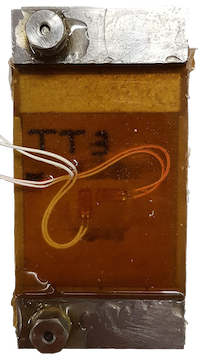
\includegraphics[width=0.4\columnwidth]{ch4/spe_coating}
    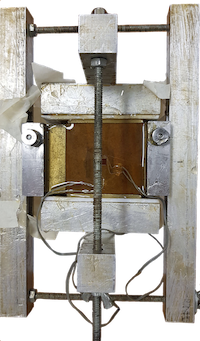
\includegraphics[width=0.4\columnwidth]{ch4/coating}
    \caption{a) Jacketed specimen and b) coating set-up}
    \label{fig4:7}
\end{figure} 

\section{Experiments} \label{ch4:exp}

Although the apparatus was designed about 30 years ago, the loading pistons were recently added to the biaxial frame. This new feature gave the possibility to explore new experiments conditions offered by the Plane-Strain Apparatus. Four tests were performed under different testing conditions and configuration of the equipment. 

\subsection{True-triaxial testing }

Since the Plane-Strain Apparatus was improved with hydraulic pistons, several true triaxial experiments, particularly under constant mean stress conditions were performed. However, none were done under plane strain conditions. One of this study objectives was to perform the first true triaxial experiment under plane strain condition in the Plane-Strain Apparatus. 

\subsubsection{Apparatus set-up}

\begin{enumerate}
    \item The specimen, coated with polyurethane, was placed on the internal load cell and the position of the axial LVDTs was adjusted. The three LVDTs and the strain gages were connected to high-pressure pass throughs located on the base unit. 
    \item The biaxial frame was then placed on the base unit, around the specimen, and the loading piston assembly put on top of the specimen and adjusted so that it was centered with the base unit. A LVDT was then attached to the linear bearing (Figure \ref{fig4:8}). 
    \item The pressure vessel was placed around the assembly, bolted with the base unit and filled with oil. 
    \item Finally, the top cap was connected to the pistons’ hydraulic circuit and bolted to the pressure vessel. 
\end{enumerate}


\begin{figure}[tb]
    \centering
    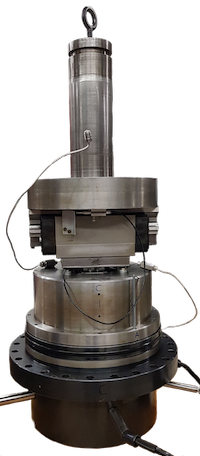
\includegraphics[width=0.4\columnwidth]{ch4/ps_setup}
    \caption{Apparatus set-up for the true-triaxial experiments}
    \label{fig4:8}
\end{figure} 

\subsubsection{Plane strain condition}

The plane strain testing condition involves control of the strain in the intermediate stress direction. As the axial (i.e. major) stress increases until failure, the intermediate stress should constantly be adjusted during the test to keep the strain constant and equal to zero in its direction.

The following procedure was applied to perform the true-triaxial experiment under the plane strain condition:  

\begin{enumerate}
    \item The Plane-Strain Apparatus was assembled, placed inside the MTS load frame the instrumentation was connected to the data acquisition system.
    \item The hydraulic intensifiers were connected to the pressure cell and the pistons. Each one was bled to ensure no entrapped air existed in the hydraulic circuit. 
    \item Seating stresses of $\sigma_1 = \sigma_2 \approx \SI{1}{MPa}$ were applied to the specimen to ensure adequate contact between the specimen and the platens. A $\sigma_3 \approx \SI{1}{MPa}$ was also applied. It is noted that this condition corresponds to a hydrostatic stress state ($\sigma_1 = \sigma_2 = \sigma_3 = \SI{1}{MPa}$).
    \item The three principal stresses were then increased hydrostatically until the desired confining pressure ($\sigma_3$) was achieved. In so doing, a stress increment of \SI{\sim 2}{MPa} was consistently used. A small deviatoric stress of about \SI{1}{MPa} was kept during the hydrostatic loading to ensure good contact between the platens and the specimen.
    \item Once the desired confining pressure (i.e. minor stress $\sigma_3$) was reached, the deviatoric loading was initiated by maintaining the minor stresses ($\sigma_3$) constant while the major stress ($\sigma_1$) was increased until failure was achieved. The intermediate stress was manually applied and controlled so that the strain in the intermediate stress direction ($\epsilon_2$) was kept constant and equal to zero during the test.  The stress path applied during the test can be summarized as follow:
\end{enumerate}

\begin{equation}
    \sigma_1 > 0 ,\quad \Delta\sigma_3 = 0 \quad \textmd{and} \quad \epsilon_2= 0
\end{equation}

he minor stress was applied using a fluid pressure system where confinement is provided using hydraulic oil. The fluid pressure system is composed of a microcontroller and a screw-type hydraulic intensifier that allows for confining pressure to be held constant throughout the test. A second hydraulic intensifier was used to apply the intermediate stress through the hydraulic pistons. The major stress was applied through the loading piston with a \SI{1}{\mega\newton} load frame. 

During the test, the following measurements were recorded: 

\begin{itemize}
    \item Internal load applied to the specimen 
    \item Axial displacement of the specimen 
    \item Axial and transversal strain of the specimen
    \item Fluid pressure applied to the specimen ($\sigma_3$ ) 
    \item Fluid pressure applied to the pistons ($\sigma_2$) 
    \item Displacement of the linear bearing
\end{itemize}

It is noted that the test was axial displacement controlled using a displacement rate of \SI{0.0005}{\meter\per\second} which was monitored from the average of the two axial LVDTs.

\subsubsection{Constant mean stress condition}


In order to compare the results given by the plane strain test, a true-triaxial experiment under constant mean stress condition was performed at the mean stress achieved at failure under plane strain condition. 

The following procedure was applied:  

\begin{enumerate}
    \item The Plane-Strain Apparatus was assembled, placed inside the MTS load frame the instrumentation was connected to the testing system.
    \item The hydraulic intensifiers were connected to the pressure cell and the pistons. Each one was bled to ensure no entrapped air existed in the hydraulic circuit. 
    \item Seating stresses of $\sigma_1 = \sigma_2 \approx \SI{1}{MPa}$ were applied to the specimen to ensure adequate contact between the specimen and the platens. A $\sigma_3 \approx \SI{1}{MPa}$ was also applied. It is noted that this condition corresponds to a hydrostatic stress state ($\sigma_1 = \sigma_2 = \sigma_3 \simeq \SI{1}{MPa}$).
    \item \emph{Hydrostatic loading phase}: The three principal stresses were then increased hydrostatically until the desired confining pressure ($\sigma_3$) was achieved. In so doing, a stress increment of \SI{\sim 2}{MPa} was used.
    \item \emph{“Deviatoric” loading phase 1}: Once the desired confining pressure (i.e. minor stress $\sigma_3$) was reached, the deviatoric loading was initiated by maintaining the minor stresses ($\sigma_3$) constant while the major ($\sigma_1$) and intermediate ($\sigma_2$) stresses were increased to the same value corresponding to the desired mean stress. The stress path applied during the phase can be summarized as follow:
    \begin{align}
        \sigma_1 = \sigma_2 = \sigma_{1,2} \; &\text{with} \; \sigma_{1,2} = 0\\
        \Delta\sigma_3 &= 0
    \end{align}
    \item \emph{“Deviatoric” loading phase 2}: Once the desired mean stress was reach, it was kept constant during the rest of the test. To do so, the minor stress was kept constant and the major and intermediate stresses followed $\Delta\sigma_1 = -\Delta\sigma_2$ until failure was achieved. 
\end{enumerate}

The lateral stresses were applied using two hydraulic intensifiers connected to the pressure vessel and the pistons. The major stress was applied through the loading piston with a \SI{1}{\mega\newton} load frame.

During the test, the following measurements were recorded: 

\begin{itemize}
    \item Internal load applied to the specimen
    \item Axial displacement of the specimen
    \item Axial and transversal strain of the specimen
    \item Fluid pressure applied to the specimen
    \item Fluid pressure applied to the pistons
    \item Displacement of the linear bearing
\end{itemize}

It is noted that the test was axial displacement controlled using a displacement rate of \SI{0.0005}{\meter\per\second}, which was monitored from the average of the two axial LVDTs.

\subsection{Axisymmetric triaxial compression experiment on a prismatic specimen}

One of the specimens prepared for an experiment under constant mean stress condition was too large to fit the biaxial frame. As the specimen preparation is time consuming, it was decided to modify the Plane-Strain Apparatus, by removing the biaxial frame, and to perform an axisymmetric triaxial compression test on a prismatic specimen. 

In this configuration, the apparatus preserved the base unit, the loading piston and the pressure cell. The axial (major) stress was still applied by the loading piston and the intermediate stress was induced through fluid pressure, equal to the minor stress. The stress state that undergoes the specimen during this experiment was similar to the one applied in conventional triaxial compression, hence the name given to the experiment (i.e. “un-conventional” triaxial compression). 

REWRITE *****In addition to the change in specimen geometry, this experiment brings a new feature to conventional triaxial compression testing, as it enables unrestricted development and propagation of the failure surface. Using this device to perform a “un-conventional” triaxial compression test was the opportunity to create new type of experiment that can bring more understanding to rock behavior at failure.*********

\subsubsection{Apparatus set-up}

For this experiment, the Plane-Strain Apparatus configuration was modified by removing the biaxial frame. In addition to the usual elements of the device, three steel cylinders equipped with threaded rod were placed between the base unit and the loading piston assembly (Figure \ref{fig3:9}). 

\begin{figure}[tb]
    \centering
    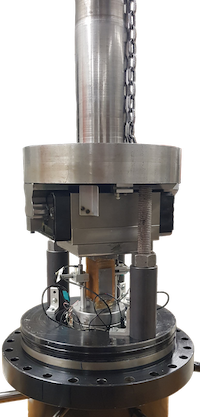
\includegraphics[width=0.4\columnwidth]{ch4/triax}
    \caption{Apparatus set-up for the “un-conventional” triaxial experiment}
    \label{fig4:9}
\end{figure} 

In the standard configuration of the device, the biaxial frame acts as an emergency stop that protects the instrumentation below the loading piston, in case of a sudden drop of the assembly due to brittle failure of the specimen. However, in this “un-conventional” triaxial testing set-up, nothing stands between the base unit and the loading piston. The three cylinders were then added to the apparatus to replace the biaxial frame and avoid damaging the instrumentation around the specimen. The height was adjusted in order to have a less than 5 \si{\milli\meter} spacing with the loading piston, which correspond to the displacement range of the LVDTs placed next to the specimen. 

As more space was available around the specimen, lateral LVDTs were also added to measure displacement and strain in the minor stress direction. 

\subsubsection{Procedure}

The procedure defined for conventional triaxial compression in Chapter \ref{ch3:title} was followed for this experiment:  

\begin{enumerate}
    \item The Plane-Strain Apparatus was assembled and placed inside the MTS load frame.

    \item  A seating stress of $\sigma_a \approx \SI{1}{MPa}$ was applied to the specimen to ensure adequate contact between the specimen and the platens. It is noted that this condition corresponds to a hydrostatic stress state ($\sigma_r = \sigma_a \approx \SI{1}{MPa}$ ).

    \item  The axial ($\sigma_a$) and radial ($\sigma_r$) stresses were then increased hydrostatically until the desired confining pressure ($\sigma_r$) was achieved. In so doing, a stress increment of \SI{\sim 2}{MPa} was consistently used.

    \item  Once the desired confining pressure (radial stress $\sigma_r$) was reached, the deviatoric loading was initiated by maintaining the radial stresses ($\sigma_r$) constant while the axial stress ($\sigma_a$) was increased until failure was achieved. The stress path applied during the test can be summarized as follow:
\end{enumerate}

\begin{align}
    \sigma_1 = \sigma_a &\text{ with } \sigma_a > 0 \\
    \sigma_2 = \sigma_3 = \sigma_r  &\text{ with } \sigma_r = 0 \\
    \sigma_a &> \sigma_r
\end{align}

$\sigma_1$, $\sigma_2$  and  $\sigma_3$  are the principal stresses of the stress state; respectively major, intermediate and minor stress.

The radial stress was applied using a fluid pressure system where confinement is provided using hydraulic oil. The axial load was applied through the loading piston with a \SI{1}{MN} MTS load frame. 

During the test, the following measurements were recorded: 

\begin{itemize}
    \item Internal load applied to the specimen 
    \item Axial and lateral displacement of the specimen 
    \item Axial and transversal strain of the specimen
    \item Fluid pressure applied to the specimen, i.e. $\sigma_3$
    \item Displacement of the linear bearing
\end{itemize}

It is noted that the test was axial displacement controlled using a displacement rate of \SI{0.0005}{\meter\per\second}, which was monitored from the average of the two axial LVDTs measurements. 

\section{Tests results}

For the purpose of this study, four experiments in the Plane-Strain Apparatus were performed: one true-triaxial test ran under plane strain condition, one “un-conventional” triaxial test and two attempts of true-triaxial test under constant mean-stress. 

\subsection{True-triaxial experiment under plane strain condition}

The true-triaxial experiment under plane strain condition was performed at with a minor stress (i.e. $\sigma_3$ ) magnitude of \SI{10}{MPa}. Table \ref{tb4:TT1} summarize the results of the experiments by presenting the stress state achieved at failure of the specimen.

\begin{table}
    \centering
    \begin{tabular}{ccccccc}
        \hline
        Test & $\sigma_1$ [\si{MPa}] & $\sigma_2$ [\si{MPa}] & $\sigma_3$ [\si{MPa}] & $p$ [\si{MPa}] & $q$ [\si{MPa}] & $\theta \si{\degree}$ \\
        \hline
        \hline
        TT1 &88.14 & 46.85 & 10 & 48.33 & 55.28 & 28.12 \\
        \hline
    \end{tabular}
    \caption{Results of the true-triaxial experiment under plane-strain condition}
    \label{tb4:TT1}
\end{table}

The stress-strain plot, presented in Figure \ref{fig4:10}, shows the evolution of the three principal stresses after the hydrostatic loading at \SI{10}{MPa}. After reaching its peak value, the axial stress decreased rapidly which reveals the brittle post-peak behavior of the rock subject to this state of stress.  By keeping $\epsilon_2 = 0$  through the test (Figure \ref{fig4:11}), the intermediate stress increased linearly until the major stress reached its peak value. At this point, failure of the specimen is achieved and the strain $\epsilon_2$ increase so does the intermediate stress. The minor stress was kept constant in accordance with the experiment requirements.

\begin{figure}[tb]
    \centering
    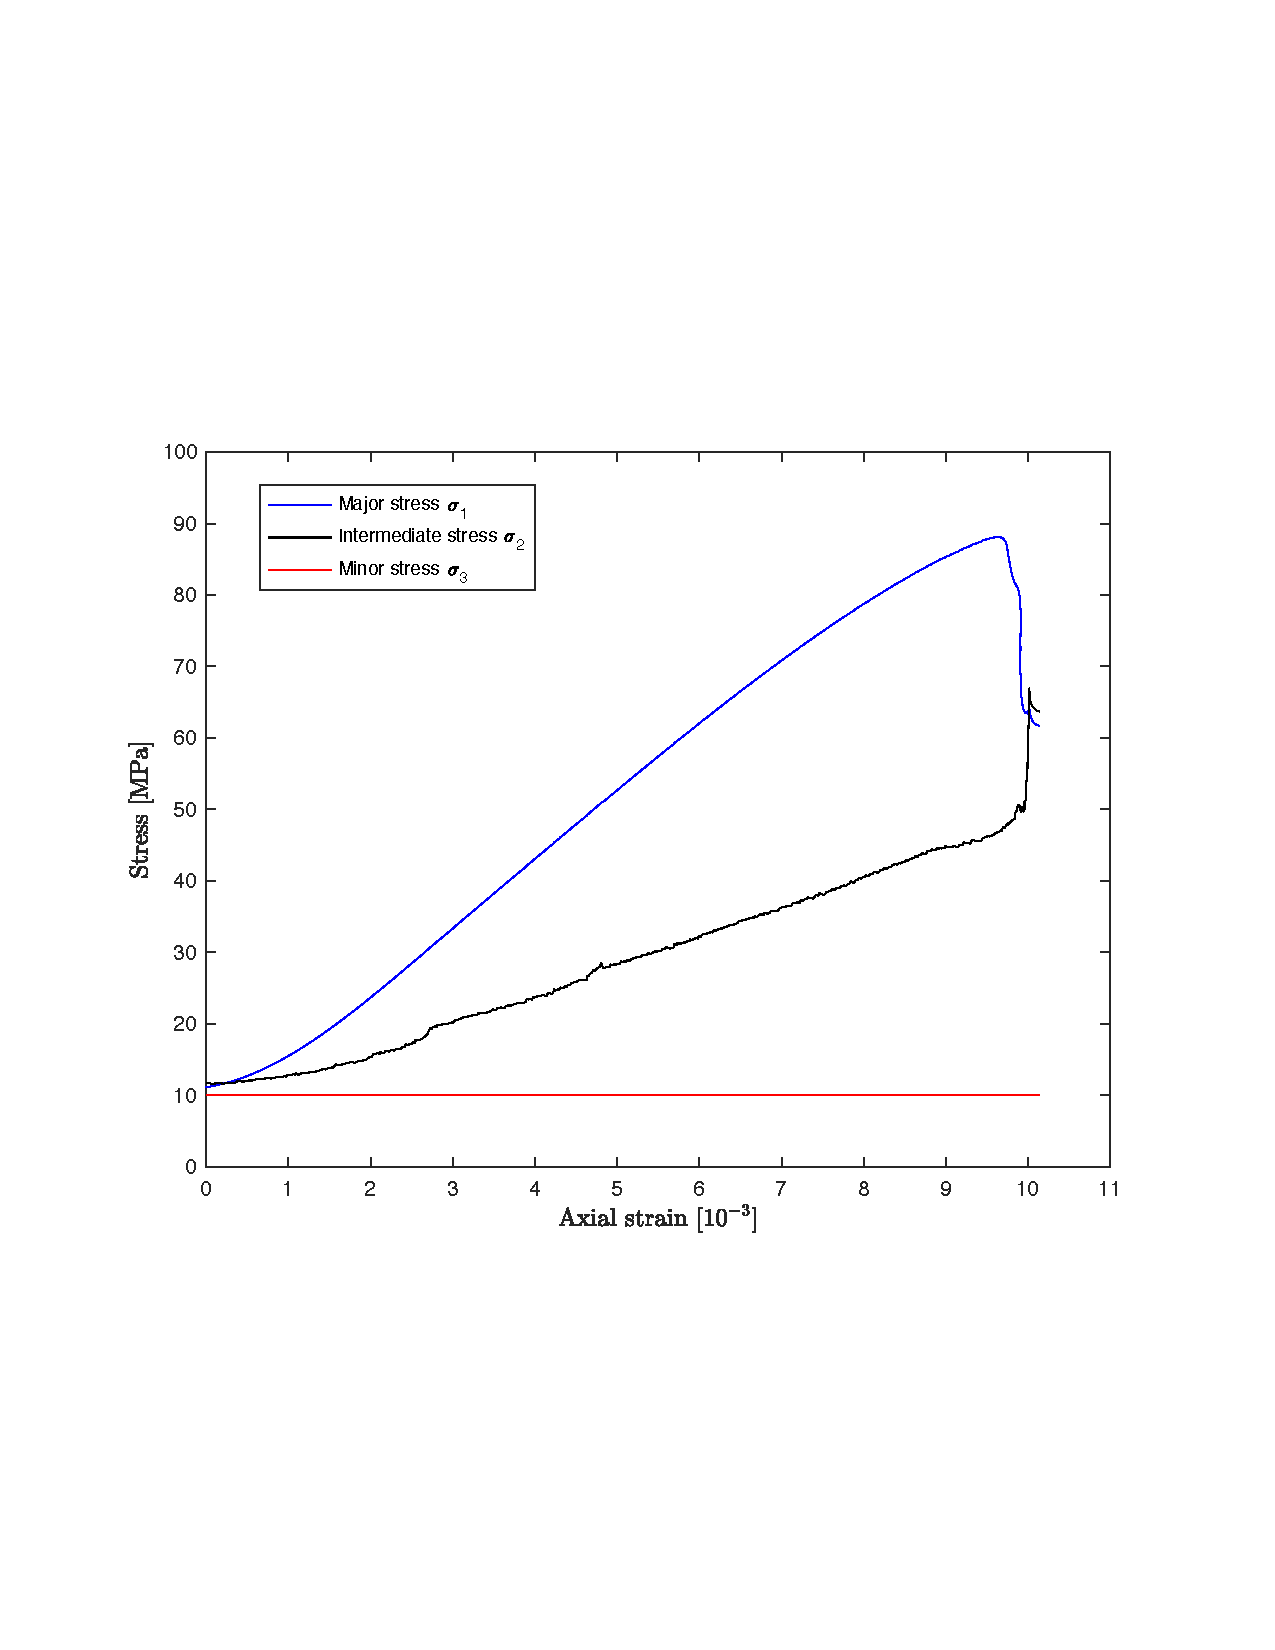
\includegraphics[width=\columnwidth]{ch4/stressvsstrain_TT1}
    \caption{$\sigma-\epsilon_a$ plot for the true-triaxial experiment performed under plane strain condition}
    \label{fig4:10}
\end{figure} 


\begin{figure}[tb]
    \centering
    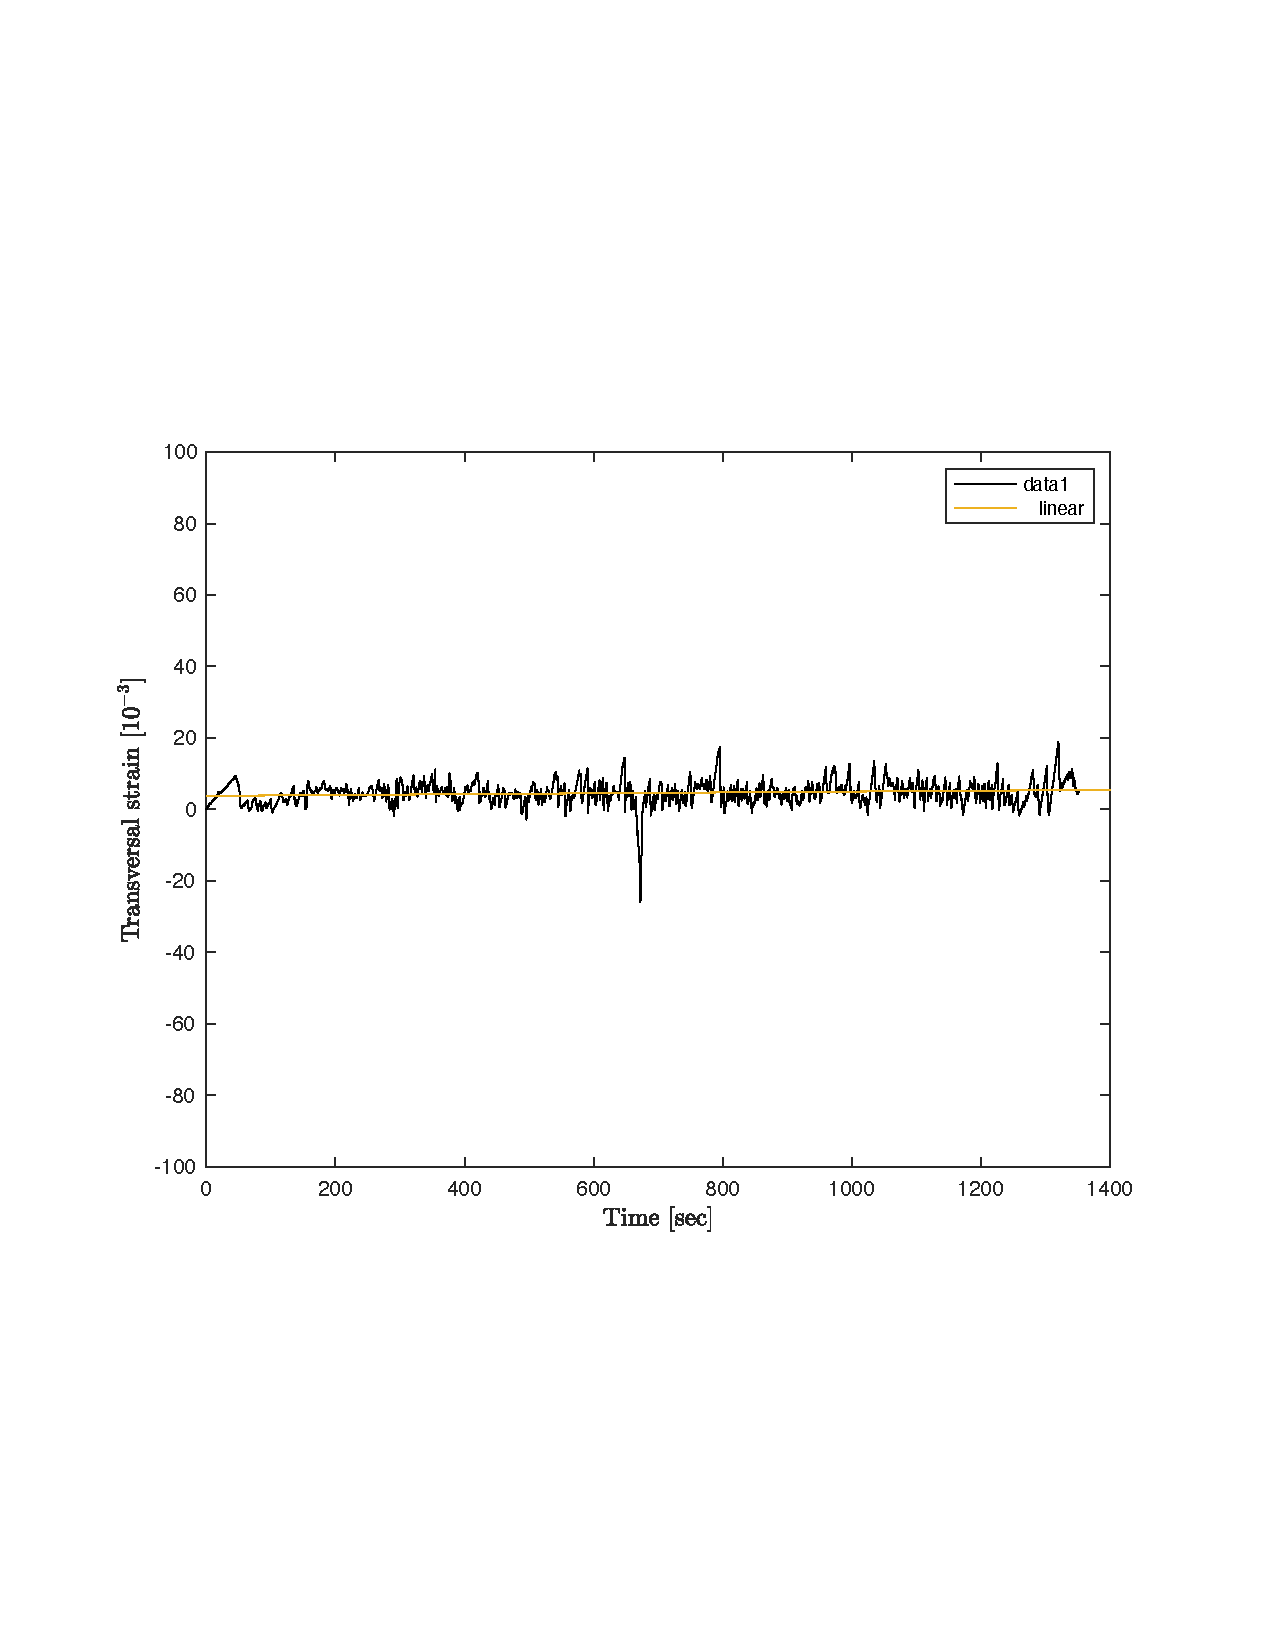
\includegraphics[width=\columnwidth]{ch4/eps2time}
    \caption{$\epsilon$ - time plot for true-triaxial experiment under plane strain condition}
    \label{fig4:11}
\end{figure} 

Figure \ref{fig4:12} shows the failed specimen the plane exposed to the pistons that applied the intermediate stress, i.e. from the ($\sigma_3$-$\sigma_1$) plane where the failure surface formed. REWRITE ********The specimen presents a kink in the failure surface at the middle of the specimen, leading to two different angles of failure (\ang{75} and \ang{65}). This “non-unique” failure angle can be explained by two different orientation of the cracks that initiated failure at the top and bottom edges of the specimen and gathered at its center.*************

\begin{figure}[tb]
    \centering
    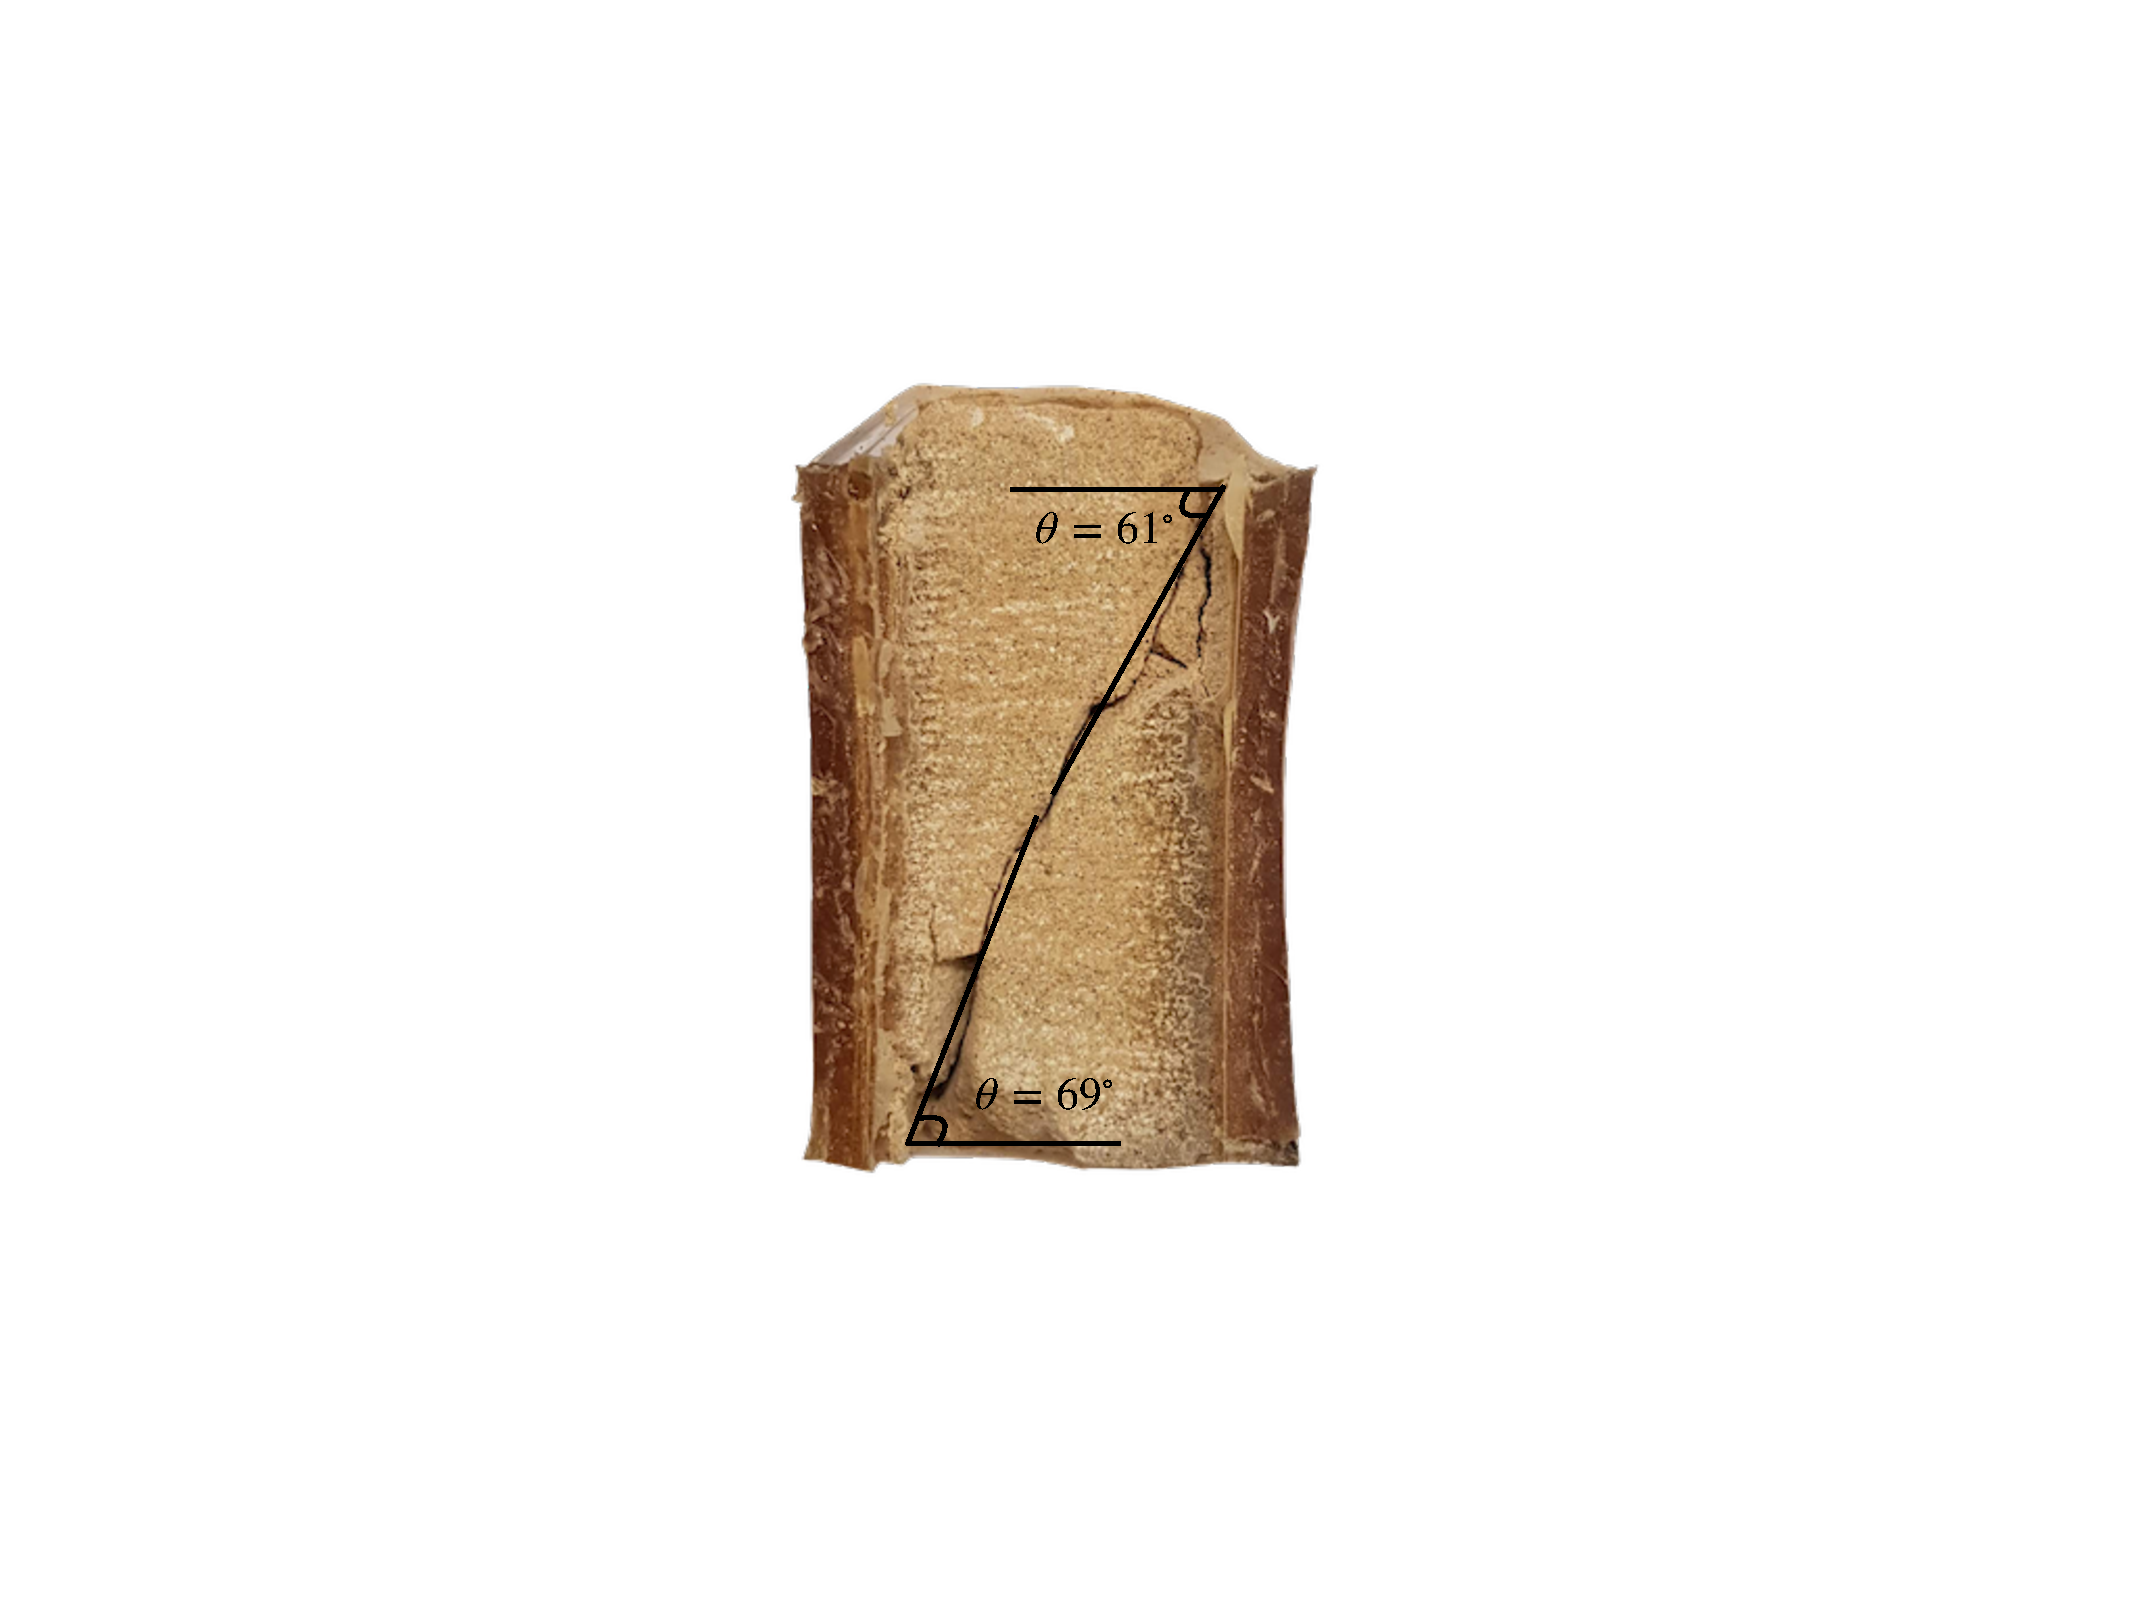
\includegraphics[width=0.4\columnwidth]{ch4/TT1}
    \caption{Failure surface of the TT 1 specimen}
    \label{fig4:12}
\end{figure} 

\subsection{“Un-conventional” triaxial experiment }

The “un-conventional” triaxial test was performed at a confining stress (i.e. $\sigma_2$ = $\sigma_3$ ) of \SI{20}{MPa}. This minor stress was chosen to be close to the highest value allowed by the pressure cell capacity, which was \SI{24}{MPa}. Table \ref{tb4:TT2} summarize the results of the experiments by presenting the stress state at achieved at failure of the specimen. 

\begin{table}
    \centering
    \begin{tabular}{ccccccc}
        \hline
        Test & $\sigma_1$ [\si{MPa}] & $\sigma_2$ [\si{MPa}] & $\sigma_3$ [\si{MPa}] & $p$ [\si{MPa}] & $q$ [\si{MPa}] & $\theta \si{\degree}$ \\
        \hline
        \hline
        TT 2 & 99.95 & 20 & 20 & 46.65 & 62.28 & 0\\
        \hline
    \end{tabular}
    \caption{Results of the axisymmetric triaxial experiment on a prismatic specimen}
    \label{tb4:TT2}
\end{table}

The stress-strain plot, presented in Figure \ref{fig4:13}, shows the evolution of the three principal stresses after the hydrostatic loading at \SI{20}{MPa}. After the axial stress reached a peak value of \SI{99.95}{MPa}, it started to decrease before stabilizing around \SI{95}{MPa} This post-peak tendency of the axial stress can be explained by the dilatancy of the specimen along the failure surface after it was formed, and the use of axial displacement control during the experiment. The minor and intermediate stresses were kept constant in accordance with the experiment conditions requirements.

\begin{figure}[tb]
    \centering
    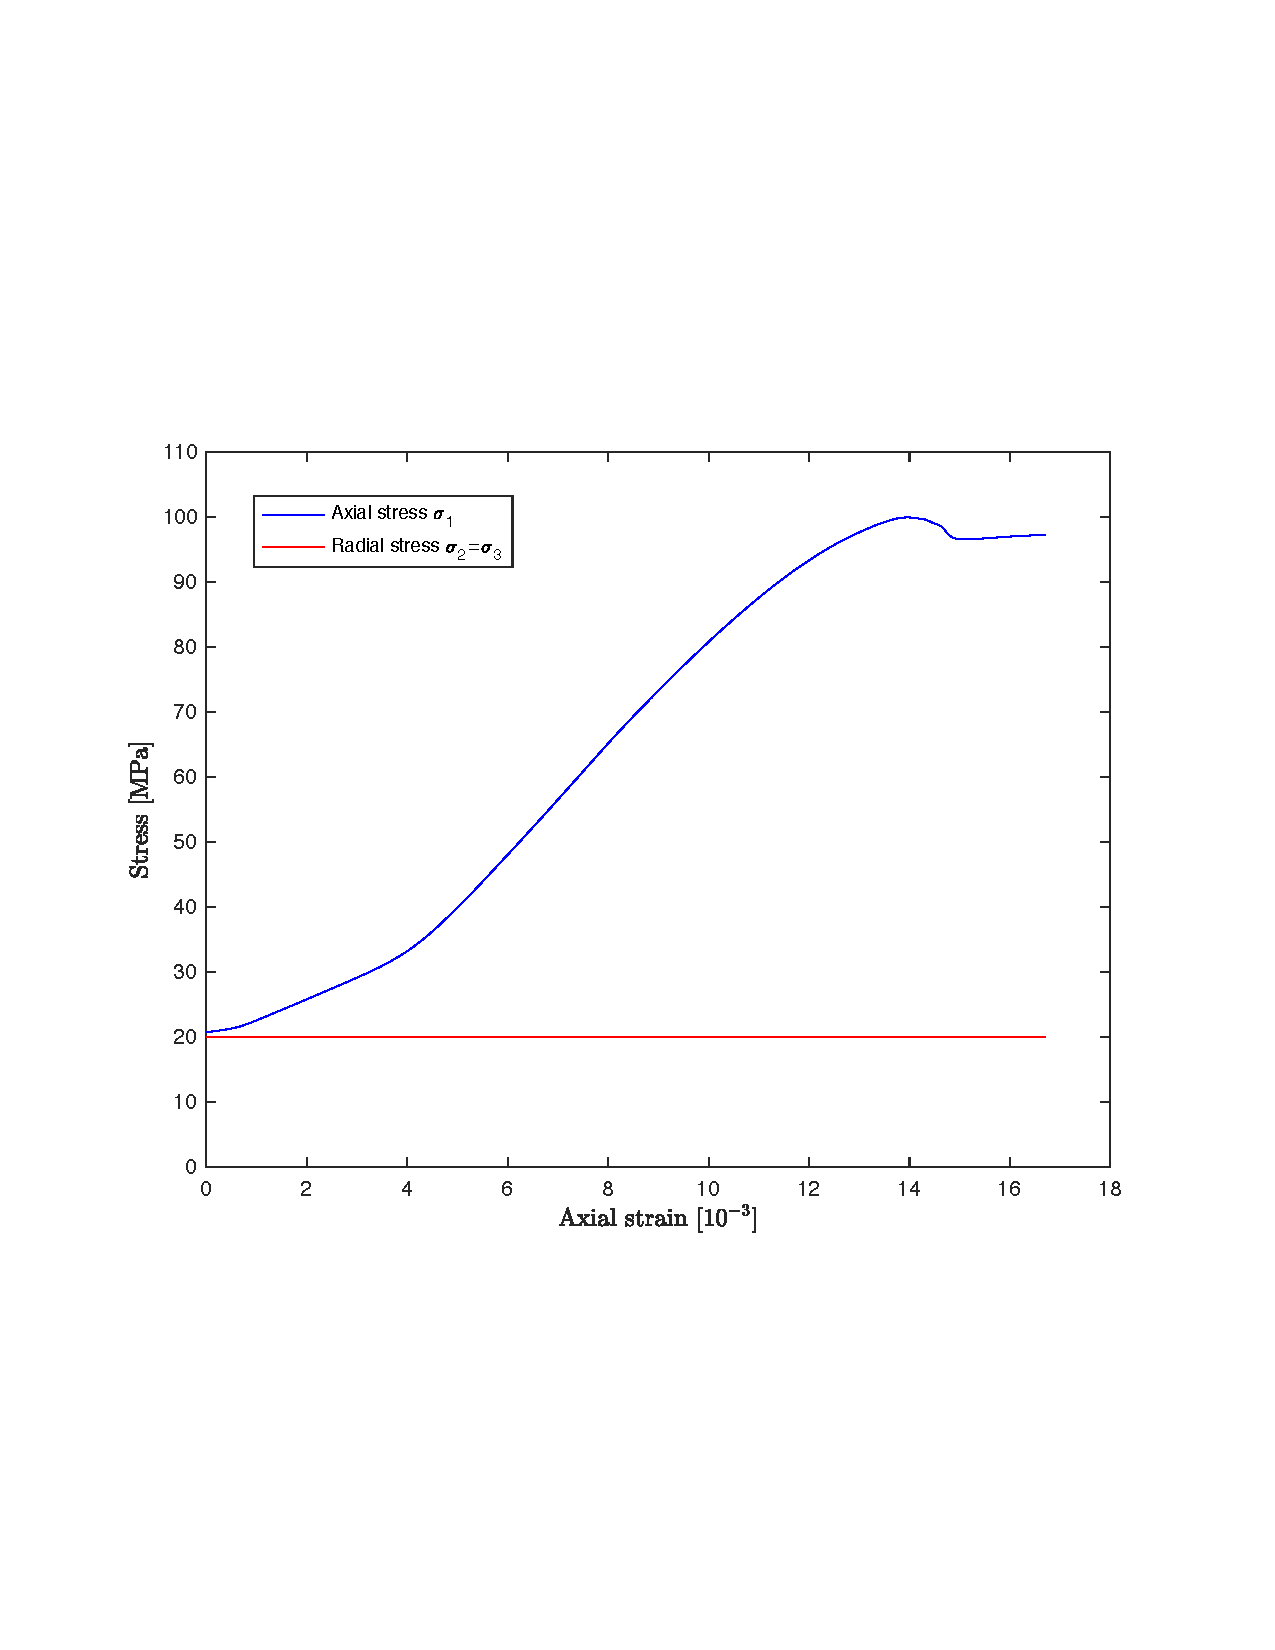
\includegraphics[width=\columnwidth]{ch4/stressvsstrain_TT2}
    \caption{$\sigma - \epsilon_a$ plot for the “un-conventional” triaxial experiment}
    \label{fig4:13}
\end{figure} 

Figure \ref{fig4:14} shows the failed specimen a) from the side perpendicular to the minor stress direction, and b) from the bottom (perpendicular to the axial stress). It presents a failure surface oriented at \ang{66}, starting from the top right and ending at the bottom middle of the specimen. 


\begin{figure}[tb]
    \centering
    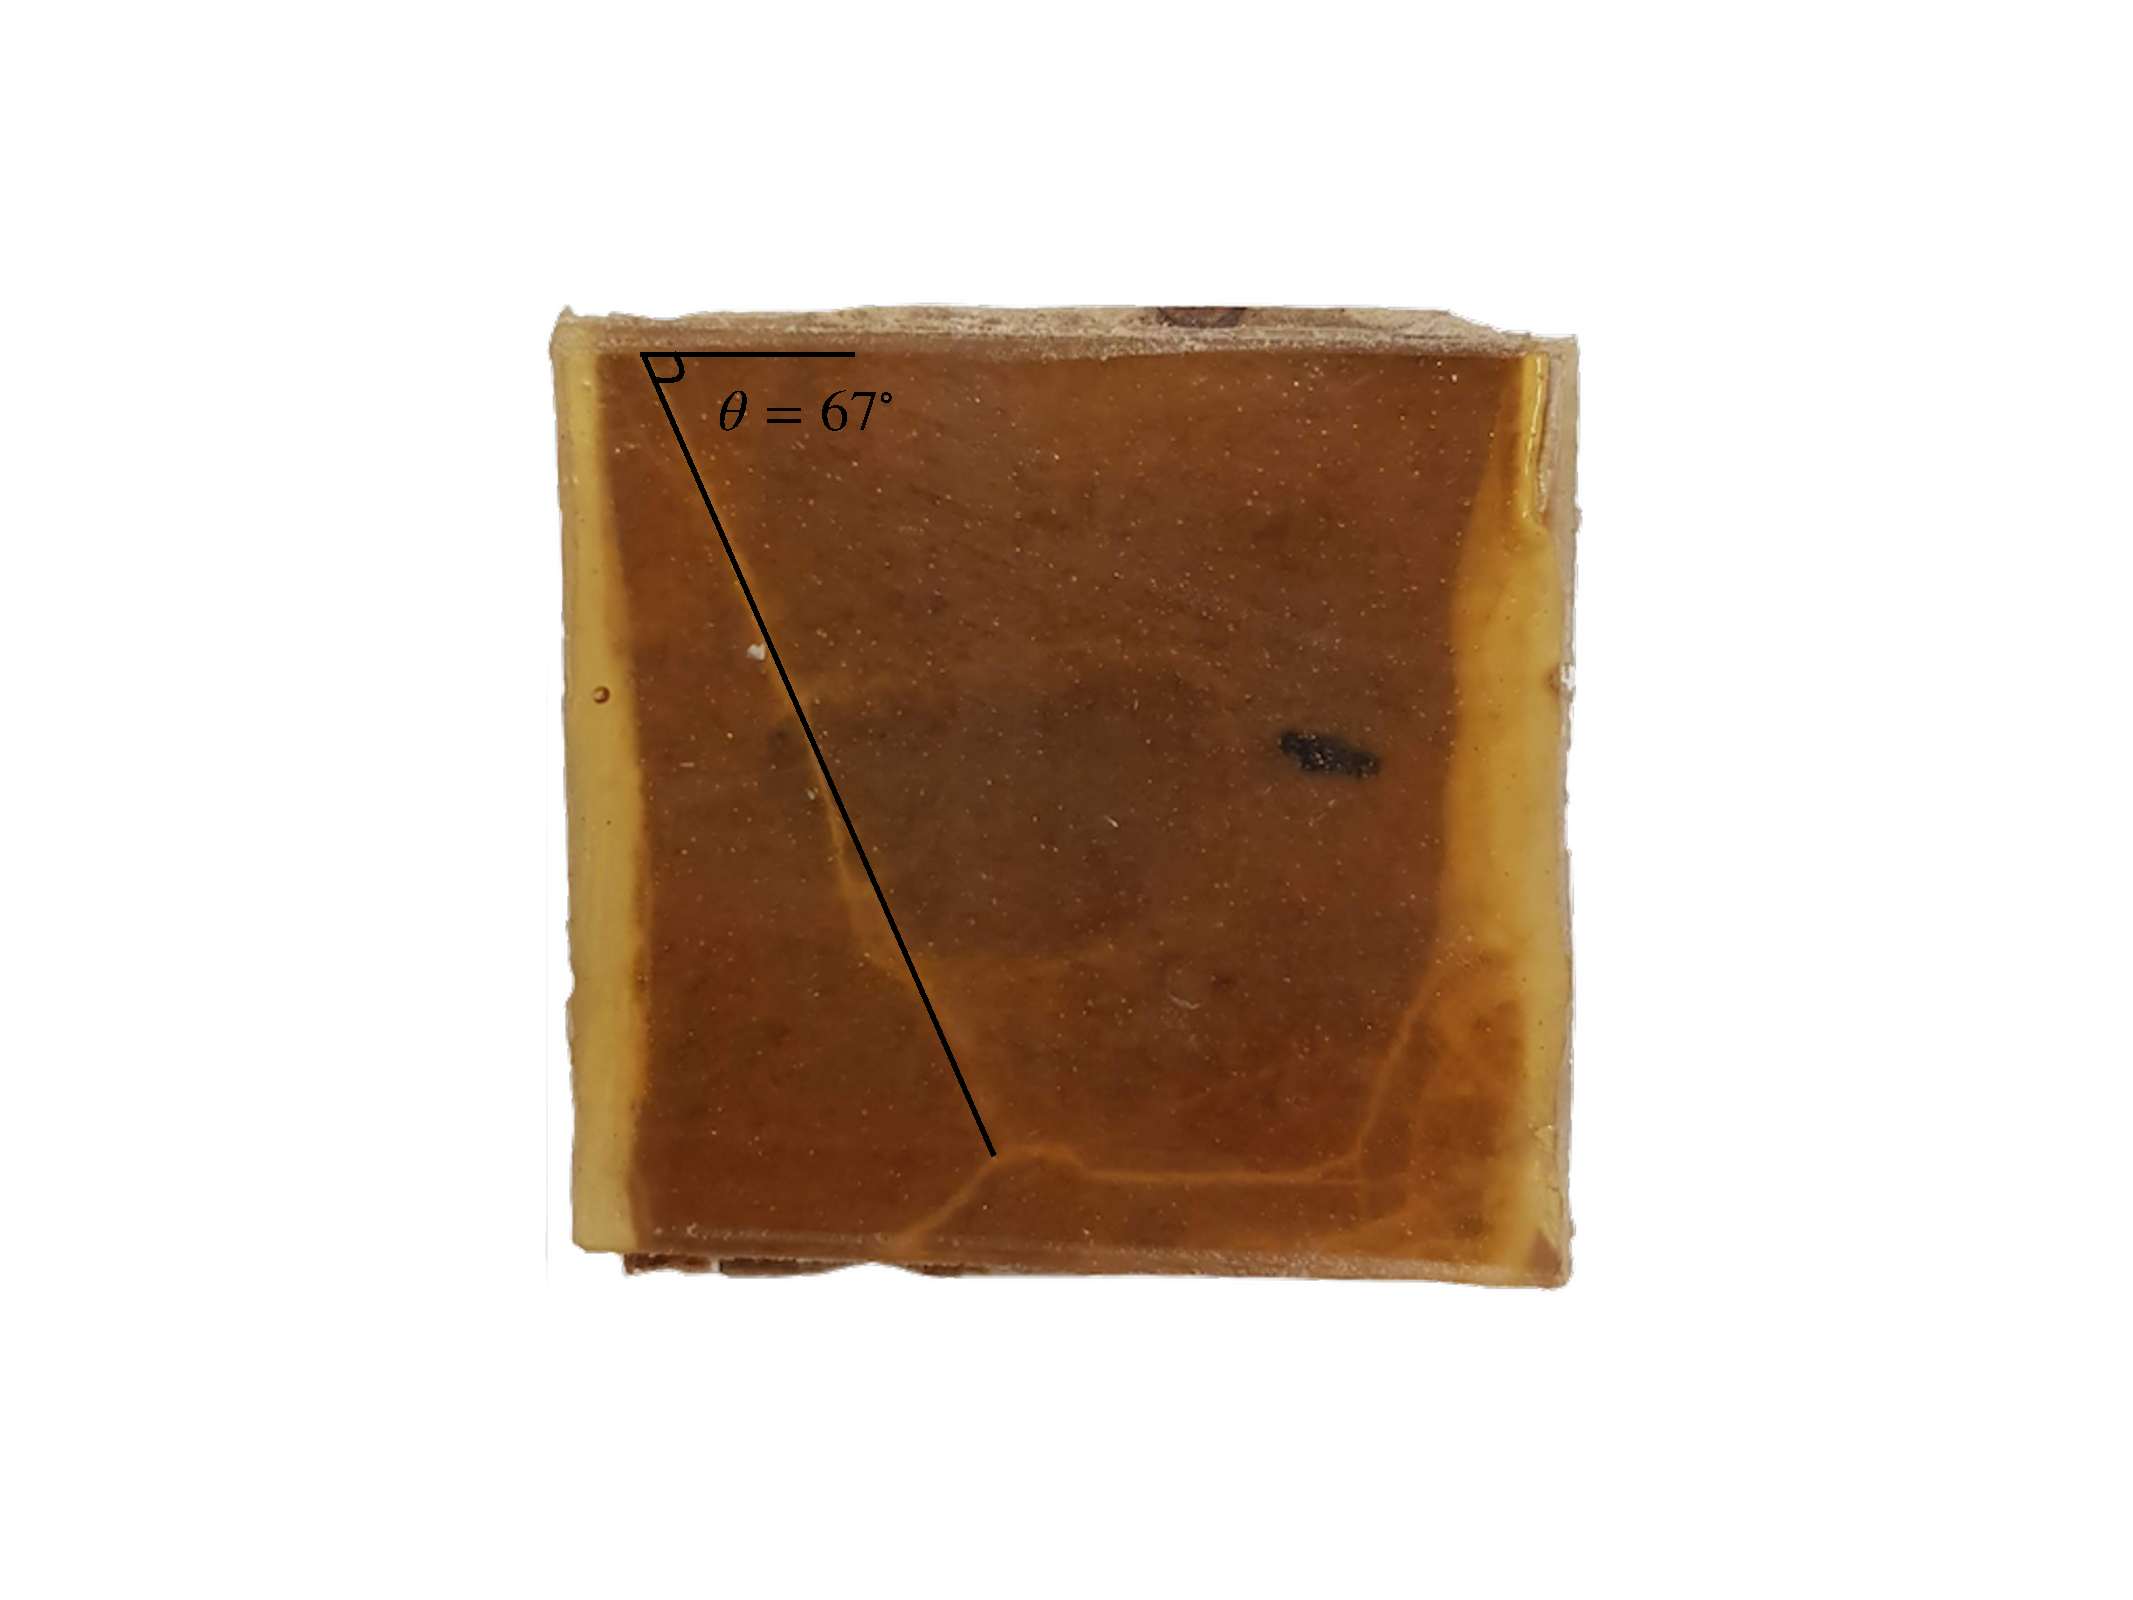
\includegraphics[width=0.4\columnwidth]{ch4/TT2}
    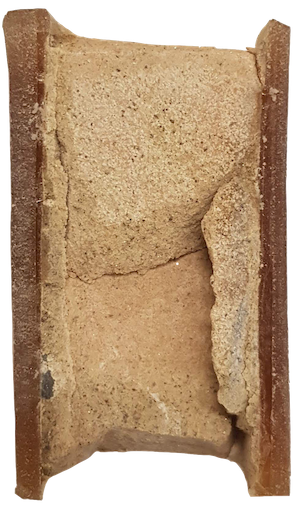
\includegraphics[width=0.2\columnwidth]{ch4/TT2top}
    \caption{Failure surface of the TT2 specimen}
    \label{fig4:14}
\end{figure} 

% For this experiment, two lateral LVDTs were added to the apparatus instrumentation. With their measurement of strain in the minor stress (i.e. $\sigma_3$ ) direction, the volumetric strain and the bulk modulus of the specimen were computed. The Bulk modulus is defined as follow:

% \begin{equation}
%     K=\frac{p}{\epsilon_V}
% \end{equation}

% where $p$  is the mean stress (cf. Equation (2.8) \ref{eq2:p2}) and  the volumetric strain. Figure \ref{fig4:15} presents the ($p$-$\epsilon_v$) plot from which the Bulk modulus was computed, giving $K = \SI{6.9}{GPa}$. 

% \begin{figure}[tb]
%     \centering
%     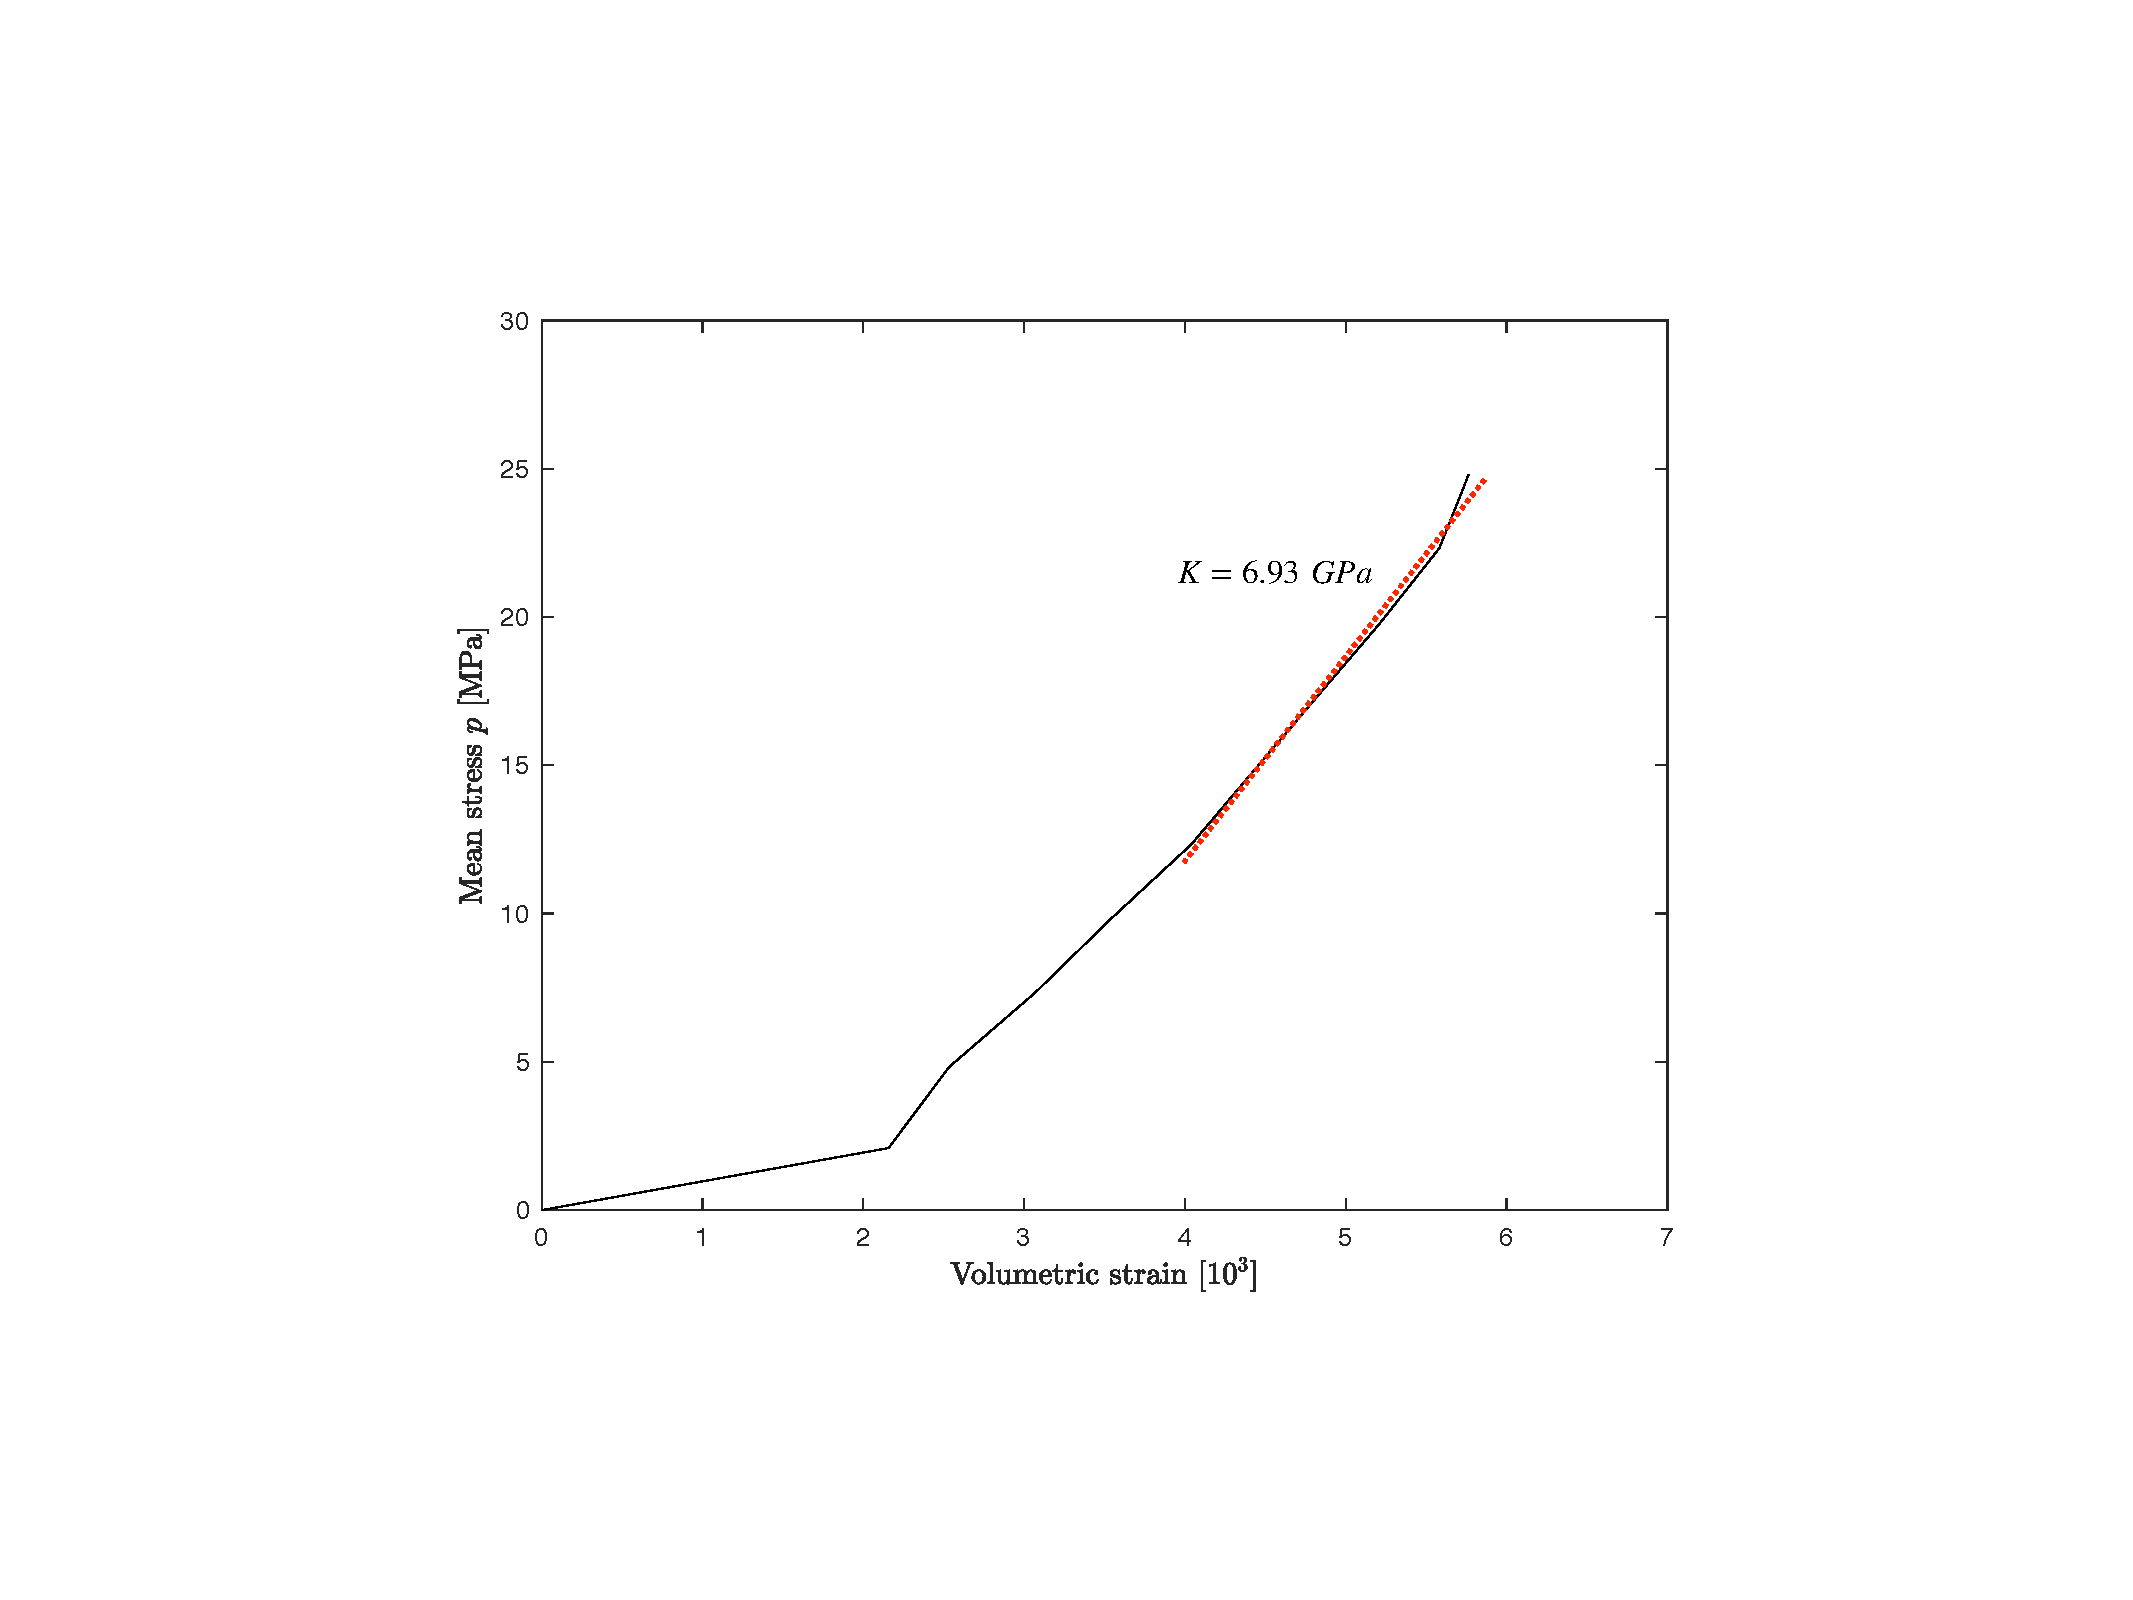
\includegraphics[width=\columnwidth]{ch4/bulkmod}
%     \caption{$p-\epsilon_V$ plot and computation of the Bulk modulus}
%     \label{fig4:15}
% \end{figure} 

A comparison with the conventional triaxial compression test performed at \SI{20}{MPa} is presented in Table \ref{tb4:TT2_CTC5}. It shows a difference of $\sim 10\%$ of axial stress at peak, the higher being reached by the prismatic specimen in the Plane-Strain Apparatus.

\begin{table}
    \centering
    \begin{tabular}{ccccccc}
        \hline
        Test & $\sigma_1$ [\si{MPa}] & $\sigma_2$ [\si{MPa}] & $\sigma_3$ [\si{MPa}] & $p$ [\si{MPa}] & $q$ [\si{MPa}] & $\theta \si{\degree}$ \\
        \hline
        \hline
        TT 2 & 99.95 & 20 & 20 & 46.65 & 62.28 & 0\\
        CTC 5 & 91.08 & 20 & 20 & 44.72 & 71.08 & 0 \\
        \hline
    \end{tabular}
    \caption{Results of the true-triaxial experiment under plane-strain condition}
    \label{tb4:TT2_CTC5}
\end{table}

\subsection{True-triaxial experiment under constant mean stress condition}

Two unsuccessful attempts to perform a true-triaxial test under constant mean stress condition were made for this study. This test results were supposed to be compared with the one of the true-triaxial test performed under plane strain condition. Therefore, the stress path followed for the test presented in this section was based on the mean stress reach at failure for $TT1$.

figure \ref{fig4:16} schematically represents the procedure defined in section \ref{ch4:exp} The initial phase is a hydrostatic loading to achieve \SI{10}{MPa}, which correspond to the minor stress applied in the first experiment. Starting from the second phase to the end, the minor stress is kept at \SI{10}{MPa}. At the end of the second phase (i.e. “deviatoric” loading phase 2), the mean stress that would be kept constant until the end of the test, is achieved. For this test, the magnitude of the major and intermediate stresses at the end of this phase were back calculated from the mean stress at failure of the first test, following Equations \ref{eq4:cstp_sig3} to \ref{eq4:cstp_init}.

\begin{equation}\label{eq4:cstp_sig3}
    p_{TT1} = \SI{44.5}{MPa} \quad \textmd{and} \quad \sigma_3 = \SI{10}{MPa}
\end{equation}
\begin{equation}
    \sigma_{1,\text{init}} = \sigma_{2,\text{init}} = \sigma_{1,2}
\end{equation}
\begin{equation}
    p_\text{initial} = \frac{2\sigma_{1,2}-\sigma_3}{2} = \SI{44.5}{MPa}
\end{equation}
\begin{equation}\label{eq4:cstp_init}
    \sigma_{1,2_{\text{int}}} = \frac{3p_\text{initial}-\sigma_3}{2} = \SI{62}{MPa}
\end{equation}
    

\begin{figure}[tb]
    \centering
    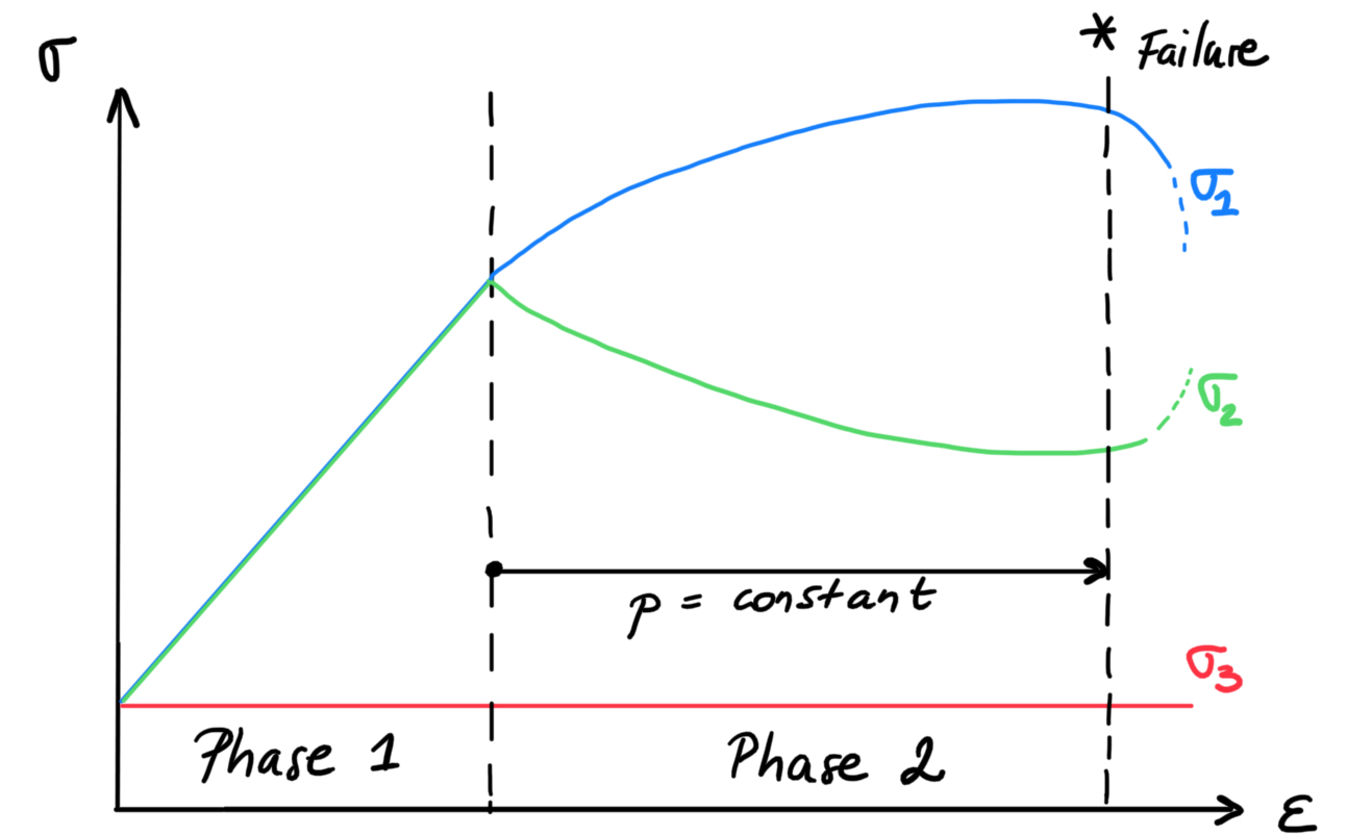
\includegraphics[width=\columnwidth]{ch4/sketch_CMS}
    \caption{Sketch of the procedure for true-triaxial experiment under constant mean stress condition}
    \label{fig4:16}
\end{figure} 

REWRITE ************ The two attempts to perform this test were stopped during this second phase. Indeed, as the major and intermediate stresses were increased at the same rate to $\sigma_{1,2} = \SI{62}{MPa}$ , $\sigma_2$ dropped the first time before reaching \SI{55}{MPa} and the second time before \SI{25}{MPa}. As suspected, they were a leak in the hydraulic pistons circuit. In the first attempt, one of them was out of its housing with the O-ring exposed and broken, and in the second, the other piston was out of its housing with the O-ring intact but exposed. 

Three possible explanations can be brought to understand what happened. The first one questions the strength and capacity of the pistons. Indeed, although the indicated maximum capacity is \SI{69}{MPa}, the first attempt showed that the leak happened before reaching this value. However, the second one leaked at low stress, and was small compared to the theoretical capacity of the pistons. The second explanation may be that the specimen failed before reaching this initialization step, which lead to think that the state of stress applied wasn’t appropriate to the rock. However, no external sign of failure has been seen on the specimen. \emph{It still might be a failure surface that we cannot see.} Finally, the third explanation may be that the specimen was not large enough, which forced the pistons to come out of their housing trying to apply a higher stress.

Although this experiment wasn't successful, previous ones performed in the Plane Strain Apparatus were. Some adjustments of the apparatus, the specimen or the procedure should be made to enable performing true-triaxial tests under constant mean stress condition. **************